% ============================================================
% main.tex — 哥本哈根留学生存手册 2026
% 仅包含文章格式、宏包与章节引用，具体内容拆分到 chapters/*.tex
% ============================================================

\documentclass[UTF8,a4paper,12pt]{ctexart}

% ------------------------------------------------------------
% 宏包与版式
% ------------------------------------------------------------
\usepackage{geometry}
  \geometry{left=2.5cm,right=2.5cm,top=2.5cm,bottom=2.5cm}

\usepackage{hyperref}
\usepackage{xurl}          % 允许长网址在更多位置换行
  \hypersetup{
    colorlinks=true,
    linkcolor=blue,
    urlcolor=blue,
    citecolor=blue
  }

\usepackage{graphicx}
  \graphicspath{{figures/}}

\usepackage{booktabs,longtable,tabularx}
\usepackage{float}          % [H] 选项
\usepackage{fancyhdr}
\usepackage{titlesec}
\usepackage{adjustbox}
\usepackage{caption}
\usepackage[normalem]{ulem} % 提供 \uline
\usepackage{enumitem}
\usepackage[dvipsnames,table]{xcolor}
\usepackage{cleveref}
\usepackage{fontspec}
\usepackage{pifont}         % ✓ ✗ ⚠

% ------------------------------------------------------------
% 自定义符号
% ------------------------------------------------------------
\newcommand{\cmark}{\textcolor{green!60!black}{\ding{52}}}   % ✓
\newcommand{\xmark}{\textcolor{red!70!black}{\ding{55}}}     % ✗
\newcommand{\warn}{\textcolor{orange}{\ding{115}}}           % ⚠

% ------------------------------------------------------------
% tcolorbox: 灰条提示框
% ------------------------------------------------------------
\usepackage{tcolorbox}
\tcbuselibrary{breakable,skins}

% 灰条提示框：左侧 3pt 灰线，可跨页
\newtcolorbox{grayleftbox}{
  enhanced,
  breakable,
  colback=white,
  boxrule=0pt,
  borderline west={3pt}{0pt}{gray!45},
  left=6pt, right=6pt, top=4pt, bottom=4pt
}

% ------------------------------------------------------------
% 页眉页脚
% ------------------------------------------------------------
\pagestyle{fancy}
\setlength{\headheight}{15pt}
\fancyhf{}
\fancyhead[L]{哥本哈根留学生存手册}
\fancyhead[R]{\leftmark}
\fancyfoot[C]{\thepage}

% ------------------------------------------------------------
% 章节标题格式
% ------------------------------------------------------------
\titleformat{\section}{\Large\bfseries}{\thesection}{1em}{}
\titleformat{\subsection}{\large\bfseries}{\thesubsection}{1em}{}

% ------------------------------------------------------------
% 强制所有 \section{} 自动换页
% ------------------------------------------------------------
\let\oldsection\section
\renewcommand{\section}{\clearpage\oldsection}

% ------------------------------------------------------------
% 文档元信息
% ------------------------------------------------------------
\newcommand{\handbookversion}{2026.4}
\newcommand{\handbookedition}{2026--2027学年版}
\newcommand{\handbookdate}{2026年8月12日}
\newcommand{\verificationdate}{2026年8月12日}

\title{哥本哈根留学生存手册\\\vspace{0.5em}\Large \handbookedition}
\author{
  \\[4em] 哥本哈根中国学生学者联合会 编辑组\\
  %\scriptsize 小编们：斯特兰奇、哥哈老油条
  % 火柿子研究所所长王卫红、出门钓鱼让二儿他妈烙了张糖饼但一条鱼没钓上于是去菜市场买了两条说是自己钓上来的二儿他爸、红豆生产达人倪斯幂会马赛回旋
  %\normal
  \\[1em]
  
\includegraphics[width=0.18\textwidth]{figures/哥哈学联Logo_圆.jpg}
  \\[4em]
}
\date{版本 \handbookversion\\发布日期：\handbookdate\\政策核验截止：\verificationdate}


% ------------------------------------------------------------
% 正文
% ------------------------------------------------------------
\begin{document}

% 控制目录仅显示到 subsection 层级（即显示 \section 和 \subsection）
\setcounter{tocdepth}{2}

\maketitle
\tableofcontents
\newpage

% ------------------------------------------------------------
% 章节引用（按需启用）
% ------------------------------------------------------------
\section{文档说明}\label{sec:docintro}


本手册由 \textbf{\href{https://cssacph.dk}{哥本哈根中国学生学者联合会（CSSA‑Copenhagen）}} 发起并持续维护，旨在为计划赴丹麦（尤其是哥本哈根地区）求学、交换或工作的同学提供 \textbf{一站式、可协作、可持续更新} 的实用信息。内容涵盖行前准备至在丹生活的方方面面，帮助大家少踩坑、多交流、快速融入～

本手册目前共有共建版和年度版两个版本。\textbf{共建版}手册为在线谷歌文档（链接： \href{https://docs.google.com/document/d/1nDohKDCMP-nRd01MiaQxyaOsbb292zW-y6yi3ryS4jo/edit?usp=sharing}{Google Doc}），欢迎所有热心的朋友分享任何在丹麦生活、工作、学习的攻略或经验。学联会定期对文档中的内容进行维护与更新。

\textbf{年度版}手册即为本PDF文档，本文档由学联编辑组整合了共建版的核心内容以及学联在微信公众号及小红书上发布的独家攻略，计划在每学年初或有重大政策变革时进行大版本更新。目前版本为 \textcolor{blue}{\textbf{2025-2026学年版}}。最近更新时间为\textcolor{blue}{\textbf{\today}}。

\begin{grayleftbox} \textbf{免责声明： }
\begin{itemize}
 \item 本手册所载信息均由学联及志愿者根据公开资料、个人经验及官方文件整理，仅供学习交流之用，不构成任何法律、医疗、签证或金融等专业建议。
 \item 由于政策、汇率及服务条款可能随时调整，我们无法保证所有内容始终最新、最完整。使用手册信息前，请务必自行向相关院校、机构及主管部门核实；因依赖本手册内容而产生的任何损失或责任，CSSA-Copenhagen 与作者团队概不承担。
 \item 若发现错误或过期信息，欢迎通过下方联系方式反馈，共同完善手册。
\end{itemize}

\end{grayleftbox}


\vspace{1em}
\textbf{联系我们：} cssa.copenhagen@gmail.com \quad\textbar\quad
欢迎扫码关注 \textcolor{ForestGreen}{\textbf{微信公众号}} \& \textcolor{red}{\textbf{小红书}}

\begin{figure}[H]
  \centering
  \setlength{\tabcolsep}{1em} % 控制两图水平间距
  \begin{tabular}{cc}
    
\includegraphics[width=0.26\linewidth]{figures/wechat_qr.png} &
    
\includegraphics[width=0.26\linewidth]{figures/xiaohongshu_qr.png} \\
    \scriptsize 微信公众号 & \scriptsize 小红书 \\
  \end{tabular}
\end{figure}

\begin{grayleftbox}
\textbf{入群信息: }

若想加入学联 2025 年丹麦留学新生群，可在学联微信公众号 \textbf{【哥本哈根 CSSA】} 或小红书 \textbf{【哥本哈根学联（CSSA）】} 后台私信，获取入群方式。
\end{grayleftbox}


\begin{grayleftbox} \textbf{内容贡献者和编者栏}
\begin{itemize}
 \item \textbf{内容贡献者：} 感谢所有为共建版手册提供内容支持的贡献者。若您希望留下姓名，可联系我们告知，我们将在之后的手册更新中列入您的名字。
 \item \textbf{学联小编（按首字母排序）：} 出门钓鱼让二儿他妈烙了张糖饼但一条鱼没钓上于是去菜市场买了两条说是自己钓上来的二儿他爸、哥哈老油条、猴子、斯特兰奇、Wen、柚子。
\end{itemize}

\end{grayleftbox}            % 序言
% ============================================
% chapters/before_departure.tex
\section{行前准备}
% ============================================

% --------------------
% Subsection: 申请流程总览（原 section 下调一级）
% --------------------
\subsection{申请流程总览}

\subsubsection{待办事项总览}

% 【子无编号小节：拿到学校 offer 后 → 下调为 paragraph*】
\paragraph*{拿到学校 offer 后}

% 灰条跨页不断裂设置（若灰条环境在下方，提前设置避免报错）
\tcbset{before skip=4pt, after skip=4pt}

% 待办事项清单（入学前）
\begin{itemize}[label=•, itemsep=2pt, leftmargin=2em]
  \item 申请住宿
  \item 缴纳学费 \& 保险
  \item 换 uncon（仅应届毕业生）
  \item 办理签证
  \item 购买机票
\end{itemize}

% 【子无编号小节：入境丹麦后 → 下调为 paragraph*】
\paragraph*{入境丹麦后}

% 待办事项清单（入境后）
\begin{itemize}[label=•, itemsep=2pt, leftmargin=2em]
  \item 按居住地规则申请 CPR，并办理 MitID、Digital Post 和黄卡；居留卡由 SIRI 或丹麦移民局制发
  \item 办理丹麦银行卡
\end{itemize}

% --------------------
% Subsection: 录取后 Checklist（原 section 下调一级）
% --------------------
\subsection{录取后 Checklist}

\subsubsection{申请住宿}
详见《留学生手册》“租房信息 \& 宿舍介绍”板块。

\subsubsection{缴纳学费 \& 保险}

% 灰条提示框（带标题）
\begin{grayleftbox}\textbf{学长学姐碎碎念}
\begin{itemize}
  \item “我在北京分行中午办的中行一类卡，需要预约，但当时很好约。”
  \item “拿到一类卡后可以买外汇，然后转到自己名下的万事达或 Visa 储蓄卡／信用卡。”
  \item “建议申请一张万事达储蓄卡（通常比 Visa 更易申请），用来境外消费和交学费。”
  \item “北京分行工作人员查看 offer 后给我开的额度很大，非常方便！”
  \item “该储蓄卡开通 POS 机免密并设置额度后几乎可当信用卡用，但每笔消费会多锁 2\% 金额，且绑卡不太方便。”
  \item “外币信用卡（如中行卓隽）可参考小红书教程申请，一张基本就够用！”
\end{itemize}
\end{grayleftbox}

\subsubsection{办理签证}
详见《留学生手册》“签证与居留许可”板块。

%\subsection{机票 \& 行李／转运}

\subsection{常见航空公司及飞行体验}

% 使用表格展示航司信息（排版紧凑，灰白条）
\begin{table}[H]
  \centering
  \scriptsize
  \renewcommand{\arraystretch}{1.2}
  \setlength{\tabcolsep}{4pt}
  \rowcolors{2}{gray!10}{white}
  \begin{tabularx}{\textwidth}{
      p{0.10\textwidth}  % 航空公司
      X  % 航线特点
      p{0.22\textwidth}  % 行李政策
      p{0.22\textwidth}  % 其他备注
    }
    \toprule
    \textbf{航空公司} & \textbf{航线特点} & \textbf{行李政策} & \textbf{其他备注} \\
    \midrule
    中国国航 &
      北京首都机场直飞哥本哈根；寒暑假票价上涨，8 月末单程约 4–5 千元；机上有 Wi-Fi &
      留学生票可托运 2 × 23 kg &
      -- \\
    泰国航空 &
      CPH出发飞 10.5 h 到曼谷；适合家在西南的同学 &
      无留学生票，只托运 1 × 23 kg &
      无 Wi-Fi；机餐好；曼谷需重新安检，勿在 CPH机场买酒 \\
    新加坡航空 &
      新加坡—哥本哈根约 13 h &
      参考官网 &
      -- \\
    汉莎航空 &
      非直达航班，整体飞行时间较长，经济舱空间一般 &
      留学生票（博士也适用）可享更多免费行李额 &
      -- \\
    \bottomrule
  \end{tabularx}
\end{table}

% --------------------
% Subsection: 入境材料（原 section 下调一级）
% --------------------
\subsection{入境材料}

% 入境材料清单
\begin{itemize}[label=•, itemsep=2pt, leftmargin=2em]
  \item 护照（含签证页）
  \item \textbf{Residence permit letter}：居留许可获批信；在居留卡尚未收到时是重要的许可证明，请保存电子版并按出入境要求携带所需材料
  \item 学校 Offer
  \item 租房合同
\end{itemize}

% 灰条提示框（带标题）
\begin{grayleftbox}\textbf{提示: }
建议所有材料携带原件及复印件各 1 份。
\end{grayleftbox}

% ----------------------- End of file -----------------------
   % 行前准备


% ============================================================
%  签证与居留许可（独立编译章节）
% ============================================================

\section{签证办理}

\subsection{阅读须知}

本章节信息仅为学联整理汇总，具体签证办理细请\textbf{务必}以丹麦移民局官网为准：

\begin{itemize}[label=•,leftmargin=2em,itemsep=2pt]
  \item 用于移民局网址：\href{https://www.nyidanmark.dk/en-GB/}{https://www.nyidanmark.dk/en-GB/}
  \item SIRI 联系方式汇总：\href{https://www.nyidanmark.dk/en-GB/Contact-us}{https://www.nyidanmark.dk/en-GB/Contact-us}


\end{itemize}


若想加入学联2025年丹麦留学新生群，获取一手信息，可在学联微信公众号【哥本哈根CSSA】或小红书【哥本哈根学联（CSSA）】后台私信，获取入群方式私信


\subsection{线上递签申请流程}

% -------- 线上递签申请流程（灰白条 + scriptsize）--------
\noindent
\scriptsize
\rowcolors{1}{gray!10}{white}           % ① 从第 3 行（数据区首行）开始灰白交替
\renewcommand{\arraystretch}{1.2}       % ② 行高微调，可按需调整
\begin{longtable}{p{0.24\linewidth}p{0.70\linewidth}}
  %\caption{线上递签申请流程}\label{tab:e-visa-steps}\\
  \toprule
  \rowcolor{gray!10} % <<< 加这一行，表头变灰
  \textbf{步骤} & \textbf{说明} \\ 
  \midrule
  \endfirsthead

  \multicolumn{2}{l}{\textit{接上页}}\\
  \toprule
  \textbf{步骤} & \textbf{说明} \\ 
  \midrule
  \endhead

  \midrule\multicolumn{2}{r}{\textit{续下页}}\\
  \bottomrule
  \endfoot

  \bottomrule
  \endlastfoot

  1. 提前准备文件 & 全本护照彩色扫描件（含封面、封底）；学校 offer；存款证明 / 学费缴纳证明（彩色扫描） \\
  2. 进入丹麦移民局签证 & \url{https://www.nyidanmark.dk/en-GB/Applying/Study} \\
  3. 选择签证类型 & 选择 \emph{Higher educational programme}（PhD选择\emph{PhD studies}），点击 \textbf{How to apply} \\
  4. 创建 case order ID & Create case order ID \\
  5. 付款（Case order ID 费用） & 约 2500 DKK，付款后务必打印 receipt \\
  6. 在线填写 ST1 表格 & 用学校邮件提供的账号密码登录；点击 \textit{"Use the online form ST1 – remember to save the screen receipt"} 完成填写，并打印 ST1 表格及回执 \\
  7. 上传所需文件 & Case ID receipt、学校 offer、学费缴费证明 / 存款证明等 \\
  8. 上传 Sworn Declaration & 系统生成宣誓证明，手写签名后扫描上传；关闭页面前再次确认已打印 ST1 表格、回执及 Case ID 收据 \\
  9. 缴纳签证费用 & \url{https://dys.um.dk/permit/} 支付约 1700 DKK；保留邮箱收到的 receipt 及 Terms \& conditions \\
  10. 14 天内采集生物信息 & 提交后 14 天内前往签证中心录指纹 / 拍照 \\
  11. 等待签证到达 & — \\

\end{longtable}
\normalsize


\paragraph{什么是 ST1 表格？}

ST1 是丹麦政府为学生居留许可设计的官方表格，分为两部分：\textbf{Part 2} 由学校填写，\textbf{Part 1} 由学生完成。仅在学生满足全部入学条件后，学校才会填写 ST1；应届生须拿到双证后尽快换 \emph{unconditional offer}，以便早日获取 ST1 并递签。

\begin{itemize}[label=•,leftmargin=2em,itemsep=2pt]
  \item 2024 年签证费：2490 DKK，建议使用 Visa 支付。
  \item 缴费后请务必截图／下载成功回执。
  \item 签证审核时长不定，建议学校发完 ST1 后尽快提交并录生物信息。
\end{itemize}

% --------------------------------------------------
\subsection{线下生物信息录入}

\subsubsection{线下递签材料准备 (From 2024)}

\tcbset{before skip=4pt,after skip=4pt}
\begin{itemize}[label=•,leftmargin=2em,itemsep=2pt]
  \item 护照原件 + \textbf{彩印}全本复印件 1 份（含空白页与封皮）+ 护照个人信息页单独 1 张
  \item 学校 con／uncon offer（建议拿到 uncon 后再递交）
  \item Tuition fee proof（学费缴费证明或存款证明）
  \item 1 张白底照片（3.5 cm × 4.5 cm）
  \item Case order ID 缴费收据
  \item 使馆签证申请费缴费收据
  \item Terms and conditions
  \item ST1 表格
  \item ST1 回执
  \item Sworn Declaration 宣誓证明
  \item 在校证明（仅 guest／exchange student 需要）
\end{itemize}

\begin{grayleftbox}{\textbf{学长学姐碎碎念}}
  \begin{itemize}
    \item 部分文件可使用无水印的手机扫描（如夸克扫描），扫描要注意确保打印出来的时候，所有页面的大小要符合实际材料的大小，否则也会要求现场重印。不过还是打印店更方便！

    \item 使馆要求 \textbf{所有材料彩印}，包括护照全本！含封面和封底。
  \end{itemize}
\end{grayleftbox}


\subsubsection{中国大陆签证中心地点}

\begin{table}[ht]
  \small
  \centering
  %\caption{中国大陆签证中心地点}\label{tab:visa-center-cn}
  \begin{tabularx}{\textwidth}{p{0.22\textwidth} X}
    \toprule
    \textbf{城市} & \textbf{地址} \\ \midrule
    北京   & 朝阳区光华路 9 号 \\
    上海   & 黄浦区四川中路 213 号 \\
    广州   & 天河区体育西路 189 号 城建大厦 3 楼 \\
    重庆   & 两江新区西湖支路 2 号 精信中心 B 塔 3 层 6 号 \\ 
    \bottomrule
  \end{tabularx}
\end{table}



\begin{grayleftbox}{\textbf{学长学姐碎碎念}}
\begin{itemize}
\item 上海下签还蛮快的，但办理时长因人而异，建议一拿到 con 就申请。
\item 如毕业证下发较晚，可请导师用学校邮箱出具可毕业证明先换 uncon（2021 年经验）。
\item 北京中心可 walk-in，约 30 分钟即可办完。
  \end{itemize}
\end{grayleftbox}


\section{居留许可 \& 黄卡申请}

新生入境后应尽快\textbf{线上预约 International House} 并\textbf{前往线下}办理居留证件，方可在丹麦正常学习、工作与生活。

\subsection{居留材料介绍}

\small
\begin{longtable}{p{0.22\linewidth}p{0.72\linewidth}}
\toprule
\rowcolor{gray!10} % <<< 加这一行，表头变灰
\textbf{材料} & \textbf{作用} \\
\midrule
\endhead
CPR number & 丹麦社会保障号，相当于身份证号码；无 CPR 无法开银行账户、就医、借书、纳税、领工资等 \\
黄卡 (sundhedskort) & 公共医疗保险卡 \& 身份证明，印有姓名、地址、CPR、家庭医生等信息；搬家需在 \href{https://lifeindenmark.borger.dk/housing-and-moving}{https://lifeindenmark.borger.dk/housing-and-moving} 更新地址并领取新黄卡 \\
粉卡 (opholdskort) & 居留卡 / ID card；非欧盟居民在丹麦合法居住的身份证明，含照片、签证类型及到期日；申根区旅行、丹麦出入境必备 \\
MitID & 丹麦国家数字身份认证系统，线上办事与支付的主要工具 \\
\bottomrule
\end{longtable}
\normalsize

\subsection{如何预约办理}

\small
\begin{longtable}{p{0.24\linewidth}p{0.70\linewidth}}
    \toprule
    \rowcolor{gray!10} % <<< 加这一行，表头变灰
    \textbf{步骤} & \textbf{说明} \\
    \midrule
    \endfirsthead
    \multicolumn{2}{l}{\textit{接上页}}\\
    \toprule
    \textbf{步骤} & \textbf{说明} \\
    \midrule
    \endhead
    \midrule\multicolumn{2}{r}{\textit{续下页}}\\\bottomrule
    \endfoot
    \bottomrule
    \endlastfoot

    1. 提前准备文件 &
      护照、居留许可 (resident permit letter)、住房合同 \\

    2. 线上申请 &
      \url{https://ihcph.kk.dk/registration-guidance/cpr-registration} \\

    3. 选择线下办理时间 &
      申请通过后，系统发送链接；选择合适时间并获取二维码／编码 \\

    4. 线下办理 &
      地址：International House Copenhagen, Nyropsgade 1, 1602 Copenhagen V \newline
      必带：护照、居留信、住房合同 \newline
      可带：学校 offer、存款证明/学费缴费证明
 \\

    5. 获得居留材料 &
      当场获得写有 CPR 号的小纸条；务必邮件告知学校 Student Service ；\newline
      黄卡、粉卡将在 2–4 周内分别邮寄至住址，请及时查收信箱 \\

    6. 激活 MitID &
      线下办理次日即可激活：下载 MitID App，按提示用护照完成激活 \\
\end{longtable}
\normalsize

% --- Comment Box -------------------------------------------------
\begin{grayleftbox}{\textbf{小贴士： }}
  \begin{itemize}
    \item 拿到 CPR 并激活 MitID 后，记得邮件告知学校，以便在学校系统里更新CPR；
    \item 搬家需及时 report 并更新黄卡地址、重新匹配家庭医生，逾期可能罚款。
    \item \textit{Digital Post} App 可查看政府来信；报税、交通罚款、青年卡政策变动等都在此处理。
    \item \textit{Sundhedskortet} App 可获得电子黄卡。
    \item 申根区旅行请随身携带护照 + 粉卡。
  \end{itemize}
\end{grayleftbox}
% ----------------------------------------------------------------





% ---------------- End of file ----------------        % DK 签证与居留许可
% ============================================================
% 抵丹后 30 天落地时间线（非欧盟学生版）
% ============================================================

\section{抵丹后 30 天落地时间线}\label{sec:arrival30}

本章默认读者是\textbf{从中国来丹、持学生居留许可的非欧盟留学生}。它把前后章节中的手续按依赖关系重新排成一条可执行时间线，适合抵丹后逐项核对。文中的“第几天”是建议节奏，并不等于统一的法定期限；实际办理速度会受住址、预约、材料和个案状态影响。

\begin{grayleftbox}
\textbf{先抓住主线：}真实且可登记的丹麦住址 $\rightarrow$ CPR 登记 $\rightarrow$ 黄卡、MitID 与 Digital Post $\rightarrow$ 银行账户和 NemKonto。居留卡由 SIRI 或丹麦移民局制发，与市民登记并行处理；税卡只在准备开始有薪工作时办理。
\end{grayleftbox}

\subsection{一张表看懂先后顺序}

\small
\rowcolors{2}{gray!10}{white}
\begin{longtable}{p{0.20\linewidth}p{0.31\linewidth}p{0.39\linewidth}}
  \toprule
  \textbf{事项} & \textbf{通常需要什么} & \textbf{办完后能做什么} \\
  \midrule
  \endfirsthead
  \toprule
  \textbf{事项} & \textbf{通常需要什么} & \textbf{办完后能做什么} \\
  \midrule
  \endhead
  \bottomrule
  \endfoot
  CPR 登记 & 真实住址、护照、非欧盟居留许可及住址证明；按个案补充家庭关系或姓名文件 & 获得丹麦个人登记号码，并进入公共医疗和数字公共服务体系 \\
  黄卡与家庭医生 & CPR 登记获批 & 系统分配家庭医生，实体黄卡通常随后邮寄；卡到之前也可凭 CPR 就医 \\
  MitID & 通常先有 CPR，并满足证件核验条件 & 登录 Digital Post、公共自助服务及许多私人服务 \\
  Digital Post & CPR 会自动开通公共机构数字信箱；访问时需要 MitID & 接收政府、税务、学校相关公共机构等具有法律效力的通知 \\
  银行账户 & CPR、住址和身份证明等；各银行审查材料不同 & 日常收付款；之后可把本人账户指定为 NemKonto \\
  NemKonto & CPR 和本人名下的丹麦或境外账户 & 接收退税、公共补助等政府付款；它不是一种新的账户 \\
  税卡 & 有薪工作信息；通常在开工前一个月内申请 & 雇主按个人税务信息预扣税；没有税卡时可能按 55\% 预扣 \\
  居留卡 & 已获批的居留许可和按要求完成的生物信息 & 作为非欧盟居民在丹居留身份的实体证明；注意它不等于 CPR \\
\end{longtable}
\normalsize

\subsection{抵丹前 4 周至出发前：把材料变成“可落地状态”}

\begin{itemize}[leftmargin=2em,itemsep=3pt]
  \item \textbf{确认住址能登记。}CPR 登记必须基于实际居住地址。向房东或宿舍确认合同、入住日期、房间号以及是否需要写 c/o；不要用并未居住的地址“挂靠”。
  \item \textbf{准备原件和电子备份。}至少包括护照、SIRI 或丹麦移民局的居留许可决定信、住址证明；如涉及婚姻、子女、改名等情况，按官方清单携带相应文件。
  \item \textbf{提前查看 CPR 入口。}居住在哥本哈根市或 International House Copenhagen 合作市镇、且满足条件者，可在线申请；最早通常可在抵达前 4 周提交，但仍须按通知本人到场核验原件。
  \item \textbf{检查生物信息与决定信。}确认已按居留许可流程录入指纹和照片，保存 Case Order ID、回执与决定信。居留许可的有效期和工作权限以决定信为准。
  \item \textbf{补齐过渡保障。}确认旅行保险或学校安排能覆盖尚未完成 CPR 登记的初期，并保存学校 International Office、住宿方和保险机构的联系方式。
\end{itemize}

\subsection{抵丹后 0--48 小时：先保证地址和身份文件可用}

\begin{enumerate}[leftmargin=2.2em,itemsep=3pt]
  \item \textbf{实际入住并立刻标好信箱。}在门铃和信箱上清楚写出自己的姓氏；使用 c/o 地址时，写法必须与申请材料一致。黄卡、居留卡和 NemKonto 激活信都可能寄到这里。
  \item \textbf{完成学校报到。}检查学生邮箱、选课和迎新通知，向学校更新丹麦手机号和联系地址；拿到 CPR 后再按学校要求更新学生档案。
  \item \textbf{分开保管重要文件。}护照、居留许可决定信及住址证明不要全部随身携带；准备一份加密电子备份。出境旅行前另查居留卡与护照要求。
  \item \textbf{核对工作权限。}学生许可所附工作权利、时数和有效期可能因项目及个案不同，任何兼职开始前都应以自己的决定信和 SIRI 当前规则为准。
\end{enumerate}

\subsection{第 1--7 天：优先完成 CPR 登记}

\begin{itemize}[leftmargin=2em,itemsep=3pt]
  \item 按 International House 或居住市镇的流程提交 CPR 登记、预约并携带原件本人到场。非欧盟学生通常要出示护照、有效居留许可和住址证明；计划在丹连续居住超过 3 个月才属于该登记路径。
  \item CPR 是个人登记号码，\textbf{不是居留许可，也不是居留卡}。即使 CPR 已办妥，仍要单独关注居留许可期限及居留卡寄送。
  \item CPR 登记获批后，系统会分配家庭医生并制作黄卡。实体卡尚未送达时，如登记已完成，通常仍可联系获分配的家庭医生就诊。
  \item 有 CPR 后尽快开通 MitID。符合护照芯片和 App 核验条件者可尝试自助开通；中国护照或手机无法完成扫描时，按 MitID 指引预约 Borgerservice/International House 核验身份，不要反复注册多个身份。
\end{itemize}

\subsection{第 7--14 天：打通数字信箱、银行与税务}

\paragraph{Digital Post}
取得 CPR 后，公共机构 Digital Post 会自动启用。用 MitID 登录并开启新信提醒，但不要只依赖提醒邮件；应主动定期检查。部分正文只提供丹麦语版本，必要时可先翻译，再向发信机构确认含义。与此同时继续查看实体信箱，因为并非所有机构都只发数字信。

\paragraph{银行账户与 NemKonto}
可开始向银行申请账户，但不同银行的材料、预约和尽职调查时间差异较大。常见材料包括护照、CPR、住址证明、录取或在读证明、居留文件以及资金来源说明。NemKonto 只是指定一个本人已有账户接收政府付款，并不要求另开一种账户：可指定丹麦账户，也可按官方流程登记境外账户。通过自助服务登记通常需要 MitID；激活信会寄往 CPR 地址，因此信箱姓名尤其重要。

\paragraph{税卡只在准备工作时办理}
没有有薪工作时，不必为了“集齐手续”提前申请税卡。已有工作合同者，通常在开工前一个月内办理；过早提交可能无法处理。符合条件时可使用 TastSelv 自助办理，否则按 SKAT 指引提交表格 04.063。雇主在没有有效税卡时可能按 55\% 预扣税，因此应在第一笔工资结算前留出处理时间。

\subsection{第 15--30 天：追踪邮寄件并做一次闭环检查}

\begin{itemize}[leftmargin=2em,itemsep=3pt]
  \item \textbf{黄卡：}CPR 登记完成后通常 2--4 周寄到。超过 4 周仍未收到，先核对信箱姓名和登记地址，再联系 Borgerservice。拿到 MitID 后也可启用 Sundhedskortet App 的电子黄卡。
  \item \textbf{居留卡：}按居留许可决定信中的主管机构追踪。若完成 CPR 登记 6 周后仍未收到，依据决定信联系 SIRI 或丹麦移民局；再次确认姓名或 c/o 已清楚标在信箱上。
  \item \textbf{银行与 NemKonto：}银行仍在审查并不罕见，保留材料清单和申请记录。如果需要接收退税或政府款项，确认 NemKonto 已成功指定，而不只是“已经有银行账户”。
  \item \textbf{学校档案：}把 CPR 按学校要求更新到学生系统；同时检查姓名拼写、地址、课程注册和考试报名是否一致。
  \item \textbf{许可自检：}在日历中记录居留许可到期日、续签准备节点和个人工作权限，不要把黄卡或 CPR 的有效状态误认为居留许可仍然有效。
\end{itemize}

\subsection{常见卡点与处理方向}

\small
\rowcolors{2}{gray!10}{white}
\begin{longtable}{p{0.28\linewidth}p{0.62\linewidth}}
  \toprule
  \textbf{卡点} & \textbf{先做什么} \\
  \midrule
  \endfirsthead
  \toprule
  \textbf{卡点} & \textbf{先做什么} \\
  \midrule
  \endhead
  \bottomrule
  \endfoot
  还没有长期住址 & 先找住宿方、学校 Housing/International Office 或所在市镇确认可登记方案。CPR 必须登记实际住址，不要使用虚假地址。 \\
  CPR 申请无进展 & 检查是否收到补材料或到场预约通知，并通过 International House/所在市镇登记部门查询；不要重复提交多个申请。 \\
  手机无法扫描中国护照 & 改走 MitID 官方提供的 Borgerservice 身份核验路径，携带有效身份证件并按预约要求准备见证人或其他材料（如适用）。 \\
  黄卡一直没到 & 登记完成 4 周后联系 Borgerservice；先检查信箱姓名和 CPR 地址。卡到前可用 CPR 联系已分配的家庭医生。 \\
  居留卡一直没到 & 查居留许可决定信确认签发机关；CPR 登记后超过 6 周仍未收到，联系 SIRI 或丹麦移民局。 \\
  银行要求反复补件 & 要求银行给出书面材料清单并保留提交记录。不同银行的客户审查不同；NemKonto 也可按官方流程指定本人境外账户。 \\
  开工前还没有税卡 & 尽快按 SKAT 指引办理并告知雇主进度；没有税卡时可能按 55\% 预扣。不要把税卡申请等同于获得工作许可。 \\
  搬家后地址仍是旧的 & 最早可在搬家前 4 周申报，最迟应在搬家后 5 天内完成地址变更；无 MitID 时联系所在市镇。 \\
\end{longtable}
\normalsize

\subsection{30 天勾选表}

\begin{itemize}[label=$\bigcirc$,leftmargin=2.2em,itemsep=3pt]
  \item 已实际入住可登记住址，信箱姓名或 c/o 与申请一致
  \item 已完成 CPR 申请、本人到场核验及学校档案更新
  \item 已确认家庭医生，并收到黄卡或知道何时向 Borgerservice 追踪
  \item 已成功登录 MitID 与 Digital Post，并设置提醒、定期主动查信
  \item 已检查居留许可期限、工作权限和居留卡寄送状态
  \item 已申请合适的银行账户；如需政府付款，已单独确认 NemKonto
  \item 如将开始有薪工作，已在合适时间申请税卡并让雇主获得税务信息
  \item 已把地址变更、续签准备和重要预约写入日历
\end{itemize}

\subsection{官方办理入口}

以下页面均为本章核验时使用的官方入口；具体材料、合作市镇和预约方式可能调整，办理当天应再次查看网页：

\begin{itemize}[leftmargin=2em,itemsep=2pt]
  \item International House Copenhagen 登记指引：\url{https://ihcph.kk.dk/registration-guidance}
  \item International House 常见问题（CPR、黄卡、居留卡）：\url{https://ihcph.kk.dk/registration-guidance/frequently-asked-questions-faq}
  \item Life in Denmark 抵丹手续总览：\url{https://lifeindenmark.borger.dk/theme/when-you-arrive}
  \item MitID 开通：\url{https://www.mitid.dk/en-gb/get-started-with-mitid/}
  \item Digital Post：\url{https://lifeindenmark.borger.dk/apps-and-digital-services/digital-post}
  \item NemKonto：\url{https://lifeindenmark.borger.dk/apps-and-digital-services/nemkonto-your-public-bank-account}
  \item SKAT 外国雇员税卡：\url{https://skat.dk/en-us/erhverv/ansatte-og-loen/udenlandsk-arbejdskraft/faa-skattekort-som-udenlandsk-medarbejder}
  \item 地址变更：\url{https://lifeindenmark.borger.dk/housing-and-moving/moving/change-address}
\end{itemize}

\noindent\textit{本章官方信息核验日期：2026 年 8 月 12 日。}
    % 抵丹后 30 天落地时间线
% ============================================
% chapters/housing.tex
\section{租房信息\&宿舍介绍}
% ============================================

% --------------------
% Subsection: 学校租房渠道（原 section 下调一级）
% --------------------
\subsection{学校租房渠道}

% --------------------
% Subsubsection: DTU校内租房网站BDTU（原 subsection 下调一级）
% --------------------
\subsubsection{DTU校内租房网站BDTU}

\noindent\textbf{官方网址：} \url{http://www.bdtu.dk}

% 【下调为 paragraph】
\paragraph{什么是 BDTU?}
Boligfonden DTU（以下简称 BDTU）是一个\textbf{私人非营利住房基金会}，专为 DTU 国际学生与国际员工（如 PhD Student、Researcher、Visiting Professor 等）提供住宿。

\paragraph{如何申请 BDTU 住房?}
\begin{enumerate}
    \item 收到 DTU 录取 offer 后，BDTU 会向新生发送一封注册邮件。
    \item 注册账号 $\Rightarrow$ 进入在线申请表，填写最多 6 个\textbf{住宿偏好}（Priority 1--6）。
    \item BDTU 尽量满足志愿，但申请人数众多，最终房源可能\textbf{并非排前几志愿}。
    \item 若满意可在邮箱中协商签署合适房源。若不满意BDTU提供的住房，可以拒绝，也可以尝试给BDTU发邮件让其安排更符合自己期望的住房
    \item 接受房源需\textbf{签署租约并支付}
    \begin{itemize}
        \item \textbf{押金}：约 2--3 月房租
        \item \textbf{首月房租}
        \item 支持银行卡或国际汇款在线支付
    \end{itemize}
\end{enumerate}

% 宿舍租金与通勤对比表格
\begin{table}[htbp]
    \scriptsize
    \rowcolors{1}{gray!10}{white}
    \centering
    \caption{BDTU各宿舍区房租与通勤对比}
    \label{tab:dorm_rent_commute}
    \renewcommand{\arraystretch}{1.2}
    \setlength{\tabcolsep}{6pt}

    % 转换为 tabularx，自动填充列宽
    \begin{tabularx}{\textwidth}{
        l  % 宿舍区
        l  % 房间类型
        X                  % 位置与通勤（自动填充）
        p{0.15\textwidth}  % 房租
    }
        \toprule
        \textbf{宿舍区} & \textbf{房间类型} & \textbf{位置与通勤} & \textbf{每月房租（不包含水电暖费用）(DKK)} \\
        \midrule
        Hempel & Single Room & 在校内，骑车 3--5 分钟，步行 5--10 分钟到教学楼 & 5198 （含水费，不含暖气和电费） \\
        Linde Alle & Single Room & 距离 DTU 约 4.5 km，骑车 15--20 分钟，公交 20--25 分钟左右到教学楼 & 4964--5302 \\
        Linde Alle & Studio & 同上 & 6415 \\
        Lundtofte & Single Room & 在 DTU 校园北部，骑车 5 分钟，步行 10--15 分钟到教学楼 & 5100 \\
        Lundtofte & Studio & 同上 & 5650--5850 \\
        Lundtofte & 2-b Apt & 同上 & 9600 \\
        Ballerup & Studio & 骑车和乘坐公交至少需 40 分钟到教学楼 & 5488 \\
        Ballerup & 2-b Apt & 同上 & 9488 \\
        U2 & Studio & 与 Lundtofte 相邻，骑车 5 分钟，步行 10--15 分钟到教学楼 & 5500 \\
        \bottomrule
    \end{tabularx}
\end{table}

\small
\noindent
\textbf{Single room}：带有卫生间（含淋浴）的单人间，厨房为多人共用。\\
\textbf{Studio Apartment}：带有卫生间（含淋浴）及厨房的单人间。\\
\textbf{2-b Apt}：带有卫生间（含淋浴）及厨房的双人间（一般为两卧室+小客厅+卫生间）。 \\
\newline
下表(表4)中提供了BDTU各宿舍区不同房型的房租与通勤对比。
 \begin{itemize}
        \item BDTU提供的住房基本都带有家具，其中Single room的实用面积大概为16-21m2，Studio大概为21-24 m2，双人间则大概为40-45 m2。
         \item 除了Hempel宿舍区的月租包含水费，表中的房租均不包含大概每月500-700 DKK的水、电、暖费用。
          \item 公交通勤时间仅为理想估计值，由于（经常）存在公交晚点的情况，所以实际乘公交通勤时间（很）可能更久。
          \item 邻居可能会在公厨开party，注重私密性建议选Studio
          \item Linde Alle步行3-6分钟即可到达Rema1000和Netto这两所超市；步行约10分钟可达Nærumvænge Butikstorv购物中心；
          \item DTU校内有一家小型的Netto超市；从宿舍区骑车5-7分钟也可到DTU南面的更大的Netto和SuperBrugse；DTU以南骑行4-5分钟就到达Lyngby购物中心。
    \end{itemize}
\normalsize

% --------------------
% Subsubsection: KU租房网站Housing Foundation（原 subsection 下调一级）
% --------------------
\subsubsection{KU租房网站Housing Foundation}

\rowcolors{0}{}{}  % 关闭灰白行染色
\begin{flushleft}
\begin{tabular}{@{}l l@{}}
\textbf{官方网站：} & \url{https://www.housingfoundation.dk} \\
\textbf{宿舍概览：} & \url{https://housingfoundation.dk/housing-options-for-student/} \\
\end{tabular}
\end{flushleft}

\paragraph{什么是 Housing Foundation?}
与哥本哈根大学（KU）合作的官方住房平台，仅限已收到 KU offer 的同学申请。
\begin{itemize}
    \item 采用“先到先得抢房”模式，新一轮房源开放时需及时查看，房间通常带基本家具。
    \item \textbf{居住时长有限}（多为半年或一年必须迁出），届时需另寻居所。
    \item 建议在\textbf{提前注册}，抢房前锁定心仪房型。
\end{itemize}

\begin{grayleftbox}\textbf{学长学姐宿舍评价（部分）}
\begin{itemize}
  \item \textbf{Bispebjerg Kollegiet： }  
  靠近北区，通勤便捷  
  近郊住宅区周边施工较吵；房间较小，偷车高发
  \item 有什么疑问可以加群问学长学姐；也欢迎大家在Google文档（链接： \href{https://docs.google.com/document/d/1nDohKDCMP-nRd01MiaQxyaOsbb292zW-y6yi3ryS4jo/edit?usp=sharing}{Google Doc}）补充入住体验
\end{itemize}
\end{grayleftbox}


% --------------------
% Subsection: 学生租房网站（原 section 下调一级）
% --------------------
\subsection{学生租房网站}

% --------------------
% Subsubsection: S.dk（原 subsection 下调一级）
% --------------------
\subsubsection{S.dk}

\noindent\textbf{官方网址：} \url{https://www.s.dk}

\paragraph{什么是 S.dk?}
\begin{itemize}
    \item 专为学生提供的租房网站，\textbf{价格低于社会房源}。
    \item 网站建议起租前 3 个月开始申请；房型含单间/双人间等，配置（公厕/私厕、公卫/私卫）不同。
    \item 通过注册后就可以自由选择排队不同的地方，排名将按照A-F的等级划分区间，A代表等级最高，即最快获得该房源。
 
\end{itemize}

\begin{grayleftbox}\textbf{小贴士： }
\begin{itemize}
  \item “可能在开学前就收到 offer，需要自行权衡是否接受。”
  \item “在获得房源offer后，如果拒绝offer将会被冻结账号，甚至封号！首次拒绝offer将被关小黑屋四周，同时其他房源的排队也将被冻结，第二次拒绝也将获得四周小黑屋！同时所有排名将被取消！”
\end{itemize}
\end{grayleftbox}

\begin{grayleftbox}\textbf{学长学姐宿舍评价（部分）}
\begin{itemize}
  \item \textbf{RNK： }  
  位于 Amager Bro，月租约 4 000 DKK，房间大，近地铁站。
\end{itemize}
\end{grayleftbox}


% --------------------
% Subsubsection: KKIK（原 subsection 下调一级）
% --------------------
\subsubsection{KKIK}

\noindent\textbf{官方网址：} \url{https://www.kollegierneskontor.dk}

\paragraph{什么是 KKIK?}
\begin{itemize}
    \item 与 s.dk 类似的学生住宿平台；建议\textbf{提前入住前 3--6 个月申请}。
    \item 官网显示设施、预计等待时间；数字排每日刷新，数字越小代表获得offer的几率越大。
    \item 规则与 s.dk 相同：一个空房源原则仅发一位申请者；拒绝offer将会被冻结账号，甚至封号！首次拒绝offer将被关小黑屋四周，同时其他房源的排队也将被冻结，第二次拒绝也将获得四周小黑屋，同时所有排名将被取消。
\end{itemize}

\begin{grayleftbox}\textbf{学长学姐宿舍评价（部分）}
\begin{itemize}
  \item \textbf{Grønjords kollegiet（绿地）:}  
   离 KU 南校步行 15 min；地铁 15 min 直达市中心；  
   月租两千多 DKK；独卫浴；公厨。

  \item \textbf{Rebæk Søpark Kollegiet (RSK):}  
  月租两千多 DKK；公厨；不在哥本哈根市区，交通卡多花一笔钱； 
  周边环境佳，周围有大草坪、小湖、森林公园和狗狗公园；  
  楼下有Lidl；步行 5–8 min 至 B 线小车 15 min 直达市区；火车上一站有netto、rema1000等；凌晨可能没有火车  
  宿舍较好排队，可能第二个工作日就下offer。
\end{itemize}
\end{grayleftbox}


% --------------------
% Subsection: 社会租房（博士/访问学者等）（原 section 下调一级）
% --------------------
\subsection{社会租房（博士/访问学者等）}

\subsubsection{租金预估（哥本哈根地区）}

% 表格保持原结构
\begin{table}[htbp]
  \small
  \centering
  \rowcolors{2}{gray!10}{white}
  \begin{tabularx}{\textwidth}{p{0.35\linewidth}p{0.3\linewidth}X}
    \toprule
    \textbf{房型} & \textbf{参考月租} & \textbf{说明} \\
    \midrule
    合租公寓单人间 & 4 000--6 000 DKK & -- \\
    小型 studio（1--2 房＋卫） & 8 000--10 000 DKK & 紧俏，适合单身/情侣 \\
    公寓（2--3 房＋卫） & 13 000--15 000 DKK & -- \\
    大型公寓（4--6 房＋卫） & 16 000 DKK 起 & 适合合租 \\
    \bottomrule
  \end{tabularx}
\end{table}

\begin{grayleftbox}\textbf{注意: }
上述房租不含水、电、网络、暖气等公用事业费，须详查租约。
\end{grayleftbox}

\subsubsection{社会房源渠道}
\begin{enumerate}
  \item \textbf{中介网站}
    \begin{itemize}
      \item 例：home、balder、EDC
      \item 流程：开放日看房 $\rightarrow$ 提交申请 $\rightarrow$ 获批签约
      \item \textbf{注意}：中介房源省事；缺点：条款死板，租金高
    \end{itemize}
  \item \textbf{宿舍学/华人微信群}
    \begin{itemize}
      \item 条件灵活；需核实信息，确认可否登记黄卡地址
    \end{itemize}
  \item \textbf{付费租房网站}
    \begin{itemize}
      \item 如 boligportal.dk（约 300 DKK/月）
      \item 可筛选条件直接联系房东
    \end{itemize}
  \item \textbf{Facebook / DBA}
    \begin{itemize}
      \item FB 群组公开透明，组织语言自我介绍成功率更高；DBA是二手网站，可设定区域筛选
      \item 私人转租应直接联系房东或合法转租人，并格外警惕诈骗
    \end{itemize}
\end{enumerate}

% 房源渠道表格保持
\begin{table}[htbp]
    \caption{可参考租房网站}    
    \scriptsize
    \renewcommand{\arraystretch}{1.15}
    \rowcolors{2}{gray!10}{white}
    \begin{tabularx}{\textwidth}{>{\raggedright\arraybackslash}X p{0.12\textwidth}
                                     >{\raggedright\arraybackslash}X p{0.12\textwidth}
                                     >{\raggedright\arraybackslash}X p{0.12\textwidth}}
        \toprule
        \textbf{网站} & \textbf{备注} &
        \textbf{网站} & \textbf{备注} &
        \textbf{网站} & \textbf{备注} \\
        \midrule
        \href{https://www.lejebolig.dk}{Lejebolig} & -- &
        \href{https://www.boligsurf.dk}{Boligsurf} & -- &
        \href{https://www.boligportal.dk}{Boligportal} & 约~300DKK/月 \\
        \href{https://housinganywhere.com}{HousingAnywhere} & -- &
        \href{https://www.home.dk}{home.dk} & -- &
        \href{https://www.dba.dk}{dba} & -- \\
        \href{https://findroommate.dk}{Findroommate} & -- &
        \href{https://cityapartment.dk}{City Apartment} & 免费 (free) &
        \href{https://housingfoundation.dk/housing-options-for-student/}{Copenhagen homes} & 免费 (free) \\
        \href{https://housingdenmark.com}{Housing Denmark} & -- &
        \href{https://propstep.com}{Propstep} & 免费 (free) &
        \href{https://lejboliger.dk}{LejBoliger} & -- \\
        \href{https://kvikbolig.dk}{Kvikbolig} & -- &
        \href{https://noliaccommodations.com}{Noli Residences} & -- &
        & \\
        \bottomrule
    \end{tabularx}
\end{table}


\begin{grayleftbox}\textbf{重要提醒: }
为保障合法权益，务必通过正规渠道签订书面租约，警惕各类骗局！
\end{grayleftbox}



% ----------------------- End of file -----------------------
            % 租房信息 & 宿舍介绍
\section{学业与校园生活}\label{sec:academic}

丹麦高校强调自主学习、课堂参与和对学习过程负责。对来自中国的非欧盟留学生而言，学业问题还可能牵动学生居留许可：选课、考试、休学或转专业，不一定只是校内事务。最稳妥的做法是同时看三层规则：\textbf{国家法规与 SIRI 居留要求、所在院校的学习规则、具体课程与考试说明}。

\begin{grayleftbox}
\textbf{本章适用前提：}默认读者是以非欧盟身份持有丹麦学生居留许可的中国留学生。若你是交换生、联合培养学生、博士生，或持有其他类型居留许可，请向本校 International Office/Student Services 与 SIRI 单独核实。
\end{grayleftbox}

\subsection{先记住：学籍状态与学生居留许可相互关联}

SIRI 要求学生居留许可持有人积极参加获准就读的课程。是否属于“active student”通常由学校根据出勤、缺席及考试通过情况等作出判断；学校也有义务向 SIRI 报告不再积极就读的学生。若不再符合条件，SIRI 可能撤销或拒绝延长居留许可。

\begin{itemize}
  \item \textbf{休学（leave of absence）：}SIRI 明确说明，一般情况下休学期间不属于积极在读。不要只在学校系统提交休学申请；应先让学校国际学生办公室说明学籍影响，并向 SIRI 核实居留后果。
  \item \textbf{退学、被退学或提前结束项目：}学生居留许可所依据的学习目的可能不再成立。学校与 SIRI 的通知可能存在时间差，不要把“居留卡尚未过期”理解为仍可合法按原条件停留。
  \item \textbf{转专业、转校或开始新项目：}不要默认原许可自动覆盖新项目。在接受新录取、缴费或办理退学前，先让 SIRI 书面确认是否需要重新申请，以及何时申请。
  \item \textbf{延期毕业：}若学习进度延误并需要延长居留，应在原许可到期前办理；SIRI 要求申请人仍在同一项目注册并积极学习。学校通常需要提供在读与学习进度信息。
\end{itemize}

官方入口：\href{https://www.nyidanmark.dk/en-GB/Words-and-concepts/SIRI/Active-student}{SIRI：Active student}、\href{https://www.nyidanmark.dk/en-GB/You-want-to-extend/Study---extension/Higher-education}{SIRI：Extend a study permit}。居留问题应以 SIRI 的个案答复为准，而不是仅凭同学经验判断。

\subsection{看懂课程、学分与学习方式}

\subsubsection*{ECTS 与学习计划}

ECTS 是欧洲高等教育常用的学分单位。丹麦常见的完整本科为 180 ECTS、两年制硕士为 120 ECTS；也存在其他长度的项目，因此\textbf{本人项目的 curriculum/programme regulations 才是毕业要求的最终依据}。制定学习计划时，不要只把 ECTS 当作课时：它通常同时覆盖上课、阅读、作业、项目与备考。

每学期选课前，至少检查以下信息：

\begin{itemize}
  \item 课程是否属于必修、限选或自由选修，能否计入本人培养方案；
  \item prerequisite（先修要求）、academic prerequisites（考试资格要求）和 mandatory activities（强制活动）；
  \item 教学语言、课程时间、校区、容量限制及是否与其他课程或考试冲突；
  \item assessment form（考核形式）、允许携带的资料/设备、评分方式及重考安排；
  \item 选课、退课、考试报名和退考的截止日期。
\end{itemize}

\begin{grayleftbox}
\textbf{容易踩坑：}课程注册不一定等于考试注册；第一次考试自动注册，也不代表重考仍会自动注册。错过退考、未出席考试或未完成强制作业，在部分院校可能占用一次考试机会。请以本校当学年的 study rules 和学生系统状态为准，并保留成功注册或退选的确认邮件/截图。
\end{grayleftbox}

\subsubsection*{常见教学形式}

\noindent\begin{tabularx}{\textwidth}{@{}p{0.24\textwidth}X@{}}
\toprule
常见名称 & 你需要做什么 \\
\midrule
Lecture & 讲授课。课前阅读与课后练习常由学生自行安排，不一定逐项提醒。 \\
Exercise class/Tutorial & 习题课或辅导课，通常用于讨论方法与解题；部分课程会把参与或提交列为考试资格。 \\
Seminar & 研讨课，常要求阅读文献、发言、展示或互评。 \\
Lab/Workshop & 实验或工作坊，可能有安全培训、出勤、实验记录和报告要求。 \\
Project/Group work & 项目或小组作业。应尽早明确分工、版本管理、引用方式及个人贡献记录。 \\
Supervision & 与导师的指导会议。提前发送议程、材料和具体问题，会比临时泛泛讨论更有效。 \\
\bottomrule
\end{tabularx}

如果英文授课节奏较快，可在第一周就向教师确认阅读优先级、课程术语与作业标准。课堂讨论中的质疑通常针对观点而非个人；清楚说明“我目前的理解是……”并提出证据，是很常见的参与方式。

\subsection{考试、成绩与申诉}

\subsubsection*{先读考试说明，再按经验备考}

丹麦高校常见闭卷/开卷笔试、口试、居家作业、项目报告、展示及组合考核。同名课程在不同学期的考试形式也可能调整。请在备考前逐项确认：

\begin{itemize}
  \item 考试日期、地点、报到要求和迟到规则；
  \item 可用资料、计算器、电脑、网络与软件，以及是否允许生成式 AI；
  \item 是否有字数/页数限制、模板、匿名提交、文件格式与命名要求；
  \item 小组成果如何认定个人贡献，口试是否基于项目报告；
  \item 突发疾病、技术故障和缺考应联系谁、在多长时间内提交何种证明。
\end{itemize}

\subsubsection*{7 分制}

丹麦目前通行的 7-point grading scale 包括 12、10、7、4、02、00 和 -3。\textbf{02 是及格线，00 与 -3 不及格}；部分课程使用 Pass/Fail（通过/不通过）或 Approved/Not approved（批准/未批准）。成绩并非简单对应中国百分制，不建议自行做线性换算；申请其他学校或工作时，优先提交正式成绩单与学校提供的评分说明。

\begin{center}
\begin{tabular}{ccl}
\toprule
成绩 & 是否通过 & 简要含义 \\
\midrule
12 & 通过 & 表现优秀，只有少量不重要的不足 \\
10 & 通过 & 表现很好，但有若干小问题 \\
7  & 通过 & 表现良好，但存在一些不足 \\
4  & 通过 & 表现尚可，但有较明显不足 \\
02 & 通过 & 达到最低可接受程度 \\
00 & 不通过 & 未达到最低要求 \\
-3 & 不通过 & 完全不可接受 \\
\bottomrule
\end{tabular}
\end{center}

国家层面的高校法规入口可见丹麦高教与科研部的\href{https://ufm.dk/en/legislation/prevailing-laws-and-regulations/education/universities}{Universities: prevailing laws and regulations}，其中包括考试与评分相关法规。丹麦文原文具有法律效力，英文版本主要用于理解。

\subsubsection*{生病、特殊安排与申诉}

\begin{itemize}
  \item \textbf{考试生病：}不要带病硬撑或事后只向任课教师解释。立即按本校流程报病，并在规定期限内提交符合要求的证明；证明形式和费用由院校规则决定。
  \item \textbf{长期疾病、残障或学习困难：}尽早联系 student counselling、study administration 或 SPS/无障碍支持。国际学生可获得的具体支持及申请材料可能不同，不要等到考试周才提出。
  \item \textbf{考试申诉：}先索取评分依据或书面决定，区分对考试过程、法律问题和学术评价的异议。高校考试法规通常规定申诉期限为结果公布后的两周，但校内提交入口和计算方式应以本校通知为准。重评或重考的结果可能低于原成绩，提交前应阅读完整后果。
\end{itemize}

\subsection{学术诚信与生成式 AI}

“只是借鉴”“组员一起写的”或“AI 帮我润色”不自动代表合规。以下行为都可能触及学术不端：未标注地复制或改写他人内容、未经允许与他人合作、重复提交自己以前的作业、伪造或选择性处理数据，以及使用考试未授权的资料或工具。

\begin{grayleftbox}
\textbf{生成式 AI 的安全判断顺序：}
\begin{enumerate}
  \item 先看具体课程页面、考试说明和本专业/学院规则是否允许；“学校总体鼓励 AI”不等于本次考试允许。
  \item 若规则不清楚，在提交前用学校邮箱向课程负责人提出具体问题，并保存书面答复。
  \item 允许使用时，按要求披露工具、版本、用途和对内容的影响；保留提示词、输出、修改记录与原始资料。
  \item 不向公共 AI 工具上传个人敏感信息、未公开研究数据、受保密协议约束的材料或他人的作品。
  \item 最终责任仍由学生承担：逐条核实事实、引用、代码、计算与参考文献，确保自己能够解释并捍卫提交内容。
\end{enumerate}
\end{grayleftbox}

不同学校甚至不同课程的界线会不同。例如，\href{https://fbu.ku.dk/english/generative-ai/}{哥本哈根大学关于生成式 AI 与良好学术实践的说明}强调诚信、透明与学生对最终成果负责；\href{https://www.ai.dtu.dk/rules/}{DTU 的 AI 规则入口}则提醒学生检查课程和考试的具体许可。它们可以帮助理解原则，但不能替代你所在院校和本次考试的规则。

小组作业建议建立简单的贡献记录：会议纪要、分工表、共享文档版本历史、代码提交记录和所用数据来源。这样既方便协作，也能在教师询问时说明个人贡献。

\subsection{学业波动时，学校与居留两条线同时处理}

\noindent\begin{tabularx}{\textwidth}{@{}p{0.18\textwidth}X X@{}}
\toprule
情况 & 校内优先动作 & 非欧盟学生额外动作 \\
\midrule
挂科或进度落后 & 联系 study adviser，核对重考、考试次数、学习活动要求与新学习计划。 & 检查是否仍会被学校认定为积极在读，以及居留到期日是否覆盖新的完成时间。 \\
考试生病 & 按时办理 sick exam/缺考证明，确认是否占用考试机会。 & 若疾病将导致长期中断或延期，向学校国际办公室与 SIRI 核实影响。 \\
考虑休学 & 先了解批准条件、复学时间、学费及校内账户权限。 & 提交申请前核实居留是否会被撤销、何时需要离境，以及复学时是否要重新申请。 \\
转专业或转校 & 获取新录取、学分转换结果和原项目结束日期。 & 让 SIRI 确认旧许可是否覆盖过渡期、是否需要新许可；不要自行假定。 \\
准备退学 & 索取书面确认、成绩单及已修学分记录。 & 立即了解合法停留基础、离境期限、住址与其他登记后续。 \\
\bottomrule
\end{tabularx}

与学校或 SIRI 沟通时，建议一次写清姓名、出生日期/案号（如适用）、学校与项目、当前学籍状态、关键日期、计划采取的动作和需要确认的问题。涉及个人信息时只使用官方渠道，不在公开群聊发布护照、居留卡或完整案号。

\subsection{新生第一个月学业清单}

\begin{enumerate}
  \item 激活学校邮箱、学生门户、学习平台和多重验证；学校正式通知通常只发到校内邮箱。
  \item 下载本人 curriculum/programme regulations 和当学年 study rules，记录文件版本与日期。
  \item 在个人日历中录入选课、退课、考试报名、退考、作业和重考截止日期。
  \item 逐门保存课程页面、learning objectives、考试形式、允许工具与 AI 说明。
  \item 核对学生系统中的课程与考试注册状态；发现异常立即用书面方式联系 administration。
  \item 找到 study adviser、International Office、student counselling、IT support 和校内紧急联系入口。
  \item 建立文件备份与引用管理习惯；重要提交保留最终文件、回执与时间戳。
  \item 检查护照和居留许可有效期，在到期前预留学校证明与 SIRI 申请时间。
\end{enumerate}

\begin{grayleftbox}
\textbf{信息核验说明：}本章国家法规与 SIRI 相关信息核验至 2026 年 8 月 12 日。院校的选课窗口、考试次数、病假证明、AI 使用和申诉入口可能每学年调整，请以学校学生门户及具体课程当期说明为准。
\end{grayleftbox}
           % 学业信息
\section{丹麦语}

\subsection{丹麦语课程介绍} \label{sec:danish}
\crefname{subsection}{节}{节}  % 输出“5.1 节”  

\subsubsection{官方丹麦语教育（Danskuddannelse）概览}
在丹麦，所有持合法居留许可、年满 18 周岁的新居民， 都可在抵达后的前 5 年内免费就读官方《丹麦语言教育》（Danskuddannelse）课程。课程由获政府许可的语言学校统一开设，最终可参加由教育部组织的全国性语言考试。

\subsubsection{课程与等级设置}
官方课程分为三条学习线，共 5–6 个模块，覆盖 CEFR A1–B2。


\begin{table}[htbp]
    \scriptsize
    \rowcolors{2}{gray!10}{white}
    \centering
    %\caption{官方丹麦语课程等级设置}
    \label{tab:danish_course_levels}
    \renewcommand{\arraystretch}{1.2}
    \setlength{\tabcolsep}{6pt}
    \begin{tabularx}{\textwidth}{l X l X}
        \toprule
        \textbf{课程线} & \textbf{适合人群} & \textbf{模块数} & \textbf{结业考试} \\
        \midrule
        DU1 & 教育背景较少的学习者 & 6 & \textit{Prøve i Dansk} 1 (PD1) \\
        DU2 & 目前参加过初中或中专教育背景 & 6 & \textit{Prøve i Dansk} 2 (PD2) \\
        DU3 & 高等教育背景、学习能力强 & 6（前 5 模块结束课后即可考试） & \textit{Prøve i Dansk} 3 (PD3) $\rightarrow$ 可继续第 6 模块并参加 \textit{Studieprøven} \\
        \bottomrule
    \end{tabularx}
\end{table}

\begin{itemize}
    \item 通过 PD3 通常可满足本地工作与部分永久居留语言要求。
    \item 通过 Studieprøven（相当于 B2/C1 后），可报考丹麦语授课高等教育项目。
\end{itemize}

\subsubsection{学习方式}
\begin{itemize}
    \item \textbf{线下固定班：} 在工作日或晚间同固定时段到校上课。
    \item \textbf{混合式（blended learning）：} 每周 1 次线下随班 + 线上自主学习。
    \item \textbf{纯线上：} 全部自选模块、讨论与作业在线完成。
\end{itemize}

\subsubsection{费用与押金政策}
\begin{itemize}
    \item 课程本身 \textbf{免费}。
    \item 首次注册需缴 2 000 DKK \textbf{押金}；按时完成模块并通过测试后，全额退还（或转入下一个模块）。
    \item 长期缺课或未在规定时间内完成模块，押金可能不予退还。
    \item 家庭团聚、au pair 等身份部分市政可免押金，具体以所在市政规定为准。
\end{itemize}

\subsubsection{课程节奏与考试}
\begin{itemize}
    \item 每个模块含定期授课、作业与期末测试；教师根据进度推荐是否参加测试。
    \item 模块测试通过后方可进入下一个模块或报名全国统一考试（PD1/PD2/PD3）。
    \item 学生可自由报名间灵活选择学习进度，\textbf{但免费资格的最长有效期为 42 个月（3.5 年）}。
\end{itemize}

\subsubsection{报名流程（通用）}
\begin{enumerate}
    \item 获取 CPR 号与激活 MitID/NemID。
    \item 在所选语言学校官网填写注册申请表，选择“Official Danish Education”。
    \item 缴纳押金，预约分级面谈（零基础可直接进入 DU3/Module 1 或 DU2/Module 1）。
    \item 依据确定的起始模块、班型与上课时间，收到欢迎邮件后按时上课。
\end{enumerate}

\subsubsection{参加资格}
\begin{itemize}
    \item 年满 18 周岁。
    \item 持有有效居留许可。
    \item 抵达后前 5 年（超过 5 年可自费就读）。
    \item 不要求入学前具备丹麦语基础。
\end{itemize}

\subsection{在大学里学丹麦语的几种途径——以 DTU 为例}

\begin{table}[htbp]
  \scriptsize
  \rowcolors{2}{gray!10}{white}
  \centering
  %\caption{语言学校上课时间示例与教学形式}
  \label{tab:danish_school_schedule}
  \renewcommand{\arraystretch}{1.2}
  \setlength{\tabcolsep}{6pt}

  % 固定宽度：学校 12%   校区 22%   上课时间 48%   形式 13%
  \begin{tabularx}{\textwidth}{p{0.12\textwidth} p{0.22\textwidth} p{0.42\textwidth} X}
    \toprule
    \textbf{语言学校} & \textbf{校区} & \textbf{上课时间示例} & \textbf{教学形式} \\
    \midrule
    Speak  & Lyngby 总校（Building 210）          & 周一–周四 17:30–19:45（每周一次线下 + 线上作业） & 混合式     \\
    UCplus & Lyngby 校区 / 纯线上                 & 晚课 17:00 起                                           & 线下或线上 \\
    Clavis & Risø 校区（Building 129）            & 周二 \& 周四 08:30–10:30                                & 线下       \\
    \bottomrule
  \end{tabularx}
\end{table}



\begin{grayleftbox}
\textbf{小提示：}
\begin{itemize}
    \item 实际时间每学期略有调整，以语言学校通知为准。    
    \item 市区的 Studieskolen 等语言中心亦接受 DTU 学生报名，居住在市区的同学可灵活选择。
    \item 所有学校均提供 \cref{sec:danish} 所述的 \textbf{官方} Danskuddannelse 课程与押金政策。
\end{itemize}
\end{grayleftbox}


\subsubsection{校内报名流程}
\begin{enumerate}
    \item 获取 CPR 号与 MitID。
    \item 在所选语言学校官网注册并注明“DTU student / staff”。
    \item 缴纳押金（与 \cref{sec:danish} 相同），预约分级测试或选择零基础班。
    \item 收到确认信后，按学校或 DTU International Student Services 指示完成学籍激活。
\end{enumerate}


\subsubsection{常用联系人与资源}
\begin{table}[htbp]
\rowcolors{2}{gray!10}{white}
\small
\centering
\begin{tabularx}{\textwidth}{lXlXlX}
\toprule
\textbf{单位} & \textbf{邮箱} & \textbf{官网} \\
\midrule
Speak (Lyngby) & \href{mailto:hello@speakspeak.dk}{hello@speakspeak.dk} & speakspeak.dk \\
UCplus (Lyngby / Online) & \href{mailto:ei@ucplus.dk}{ei@ucplus.dk} & ucplus.dk \\
Clavis (Risø) & \href{mailto:kontakt@clavis.org}{kontakt@clavis.org} & clavis.org \\
DTU International Student Services & \href{mailto:iss@dtu.dk}{iss@dtu.dk} & dtu.dk/international \\
\bottomrule
\end{tabularx}
\end{table}

%\vspace{1ex}
如需注册/押金、课程结构等通用细节，请参见 \textbf{\cref{sec:danish} 丹麦语课程介绍}。
             % DK 丹麦语学习
%============================================================
% 6. 交通
%============================================================
\section{交通}\label{sec:traffic}

\subsection{哥本哈根公共交通介绍}

\subsubsection{巴士}
遍布整个首都地区，贯穿哥哈城区的主要交通方式之一。可在巴士上向司机购买单程票，或提前在车站自动售卖机与线上 APP 购买车票。站台及 APP 可实时查看到站时间。

\subsubsection{地铁}
主要覆盖市中心／机场（1–4 区）。\textbf{必须在上车前持有有效车票}；四条线路 \texttt{M1\textendash M4}。详见官网：
\url{https://www.m.dk/rejser/se-metroens-linjer/}

\subsubsection{城郊火车（S-tog）}
遍布首都大区，以字母+终点站区分线路。\textbf{上车前须持票}。线路图：
\url{https://www.dsb.dk/s-tog/}

\subsubsection{城际火车（regional tog）}
连接丹麦主要城市，现场或线上购票：
\url{https://www.dsb.dk/}

\subsubsection{黄色火车（Lokaltog）}
服务哥本哈根地区：\url{https://www.lokaltog.dk}

\subsubsection{轻轨（建设中）}
预计 2025 年通车，Lyngby–Ishøj 方向：
\url{https://www.dinletbane.dk}

%------------------------------------------------------------
\subsection{交通卡 \textit{Rejsekort} 办理}\label{sec:rejsekort}

\begin{itemize}[leftmargin=1.5em]
  \item 线下机可办\textbf{匿名卡}（70 DKK），线上/APP 办\textbf{实名卡}（20 DKK）。
  \item 乘车前 \textit{Check-in}，下车 \textit{Check-out}，按区数计费；比单程票便宜（单程最低 24 DKK）。
  \item 卡片类型  
        \begin{itemize}
            \item \textbf{实名卡}：仅本人使用，优惠最大，可邮寄到家；  
            \item \textbf{匿名／灵活匿名卡}：后者可借他人且享一定优惠，可官网下单。
        \end{itemize}
\end{itemize}

\begin{figure}[htbp]
    \centering
    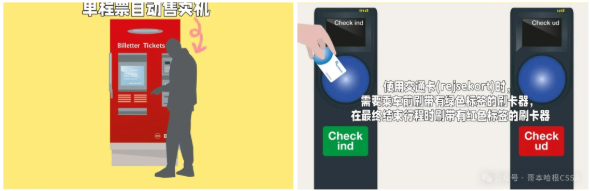
\includegraphics[width=.9\linewidth]{figures/rejsekort_machine.png}
    \caption{单程票售票机与 Rejsekort 打卡示意}
\end{figure}

%------------------------------------------------------------
\subsection{交通 APP}\label{sec:traffic-app}

\begin{figure}[htbp]
    \centering
    
\includegraphics[width=.7\linewidth]{figures/transport_apps.png}
    \caption{常见公共交通 APP（左起：Rejseplanen、DSB、DOT、RejseBillet）}
\end{figure}

\subsubsection{Rejseplanen}
查询全部公共交通线路与实时到站／延误。

\subsubsection{DOT}
购单程票、月票、通勤卡，激活青年卡。

\subsubsection{DSB}
城际火车购票；支持月票、往返瑞典南部月票等。

\begin{grayleftbox}
\textbf{学长学姐碎碎念 }
\begin{itemize}
  \item 我拥护 DSB!!，非高峰自带折扣，信用卡协议免验证。购票或充值可获 7-11 积分，免费兑换吃喝。
\end{itemize}
\end{grayleftbox}

\subsubsection{RejseBillet}
2023 新 APP，与 DOT 功能重叠，未来可能整合。

%============================================================
% 7. 购物
%============================================================
\section{消费 \& 购物}

\subsection{二手交易平台}
\begin{itemize}
  \item \textbf{DBA}
  \item \textbf{Facebook Marketplace}
  \item \textbf{微信群}
\end{itemize}

\subsection{日常消费App推荐}
\begin{itemize}
  \item \textbf{MineTilbud} — 超市打折聚合 APP  
  \item \textbf{Lidl Plus} — 会员折扣+积分  
  \item \textbf{Netto+ Scan \& Go} — 免排队、免国内卡手续费  
  \item \textbf{Too Good To Go} — 盲盒 app，冬天囤早餐食材
\end{itemize}

% ============================================
% chapters/bank_cards.tex
% 银行卡主流选项对比（层级统一下调版）
% ============================================

% --------------------
% Subsection: 银行卡主流选项对比
% --------------------
\subsection{银行卡}

% --------------------
% Subsubsection: 关键办理要点
% --------------------
\subsubsection{关键办理要点}

\begin{enumerate}[leftmargin=3em,label=\arabic*.]
  \item \textbf{必备文件}\\
        护照、丹麦 CPR 号（黄卡）、居留许可、MitID 是所有银行通用硬指标。线上或线下银行均可能核对这些信息。
  
  \item \textbf{开户速度}\\
        \textbf{Revolut/Lunar}：视频或自拍认证后即刻得到虚拟卡，实体卡 3–7 天寄达。\\
        \textbf{传统银行}：在线申请 → 邮件/电话排队 → 线下面谈（约 30 min）→ 等待后台审批，整体 1–4 周不等。
  
  \item \textbf{费用 \& 账户维护}\\
        学生套餐多为 0 DKK/月，但超过年龄／毕业后可能转为普通账户；少数银行会收取季度费。使用前确认收费及变更条款。
  
  \item \textbf{多币种与外汇}\\
        \textbf{Revolut}：36 种即时汇兑，适合从人民币汇款兑换 DKK。\\
        \textbf{Lunar/Danske} 等本地银行多币功能有限，跨境电汇手续费 50–75 DKK 起。
\end{enumerate}

% 银行对比表
\subsubsection{留学生部分常见银行卡对比}
\begin{table}[H]
  \scriptsize
  \rowcolors{2}{gray!10}{white}
  \centering
  %\caption{中国}
  \label{tab:bank_compare_new}
  \renewcommand{\arraystretch}{1.25}
  \setlength{\tabcolsep}{5pt}
  \begin{tabularx}{\textwidth}{p{0.12\textwidth} p{0.09\textwidth} p{0.13\textwidth} p{0.15\textwidth} X X}
    \toprule
    \textbf{银行/账户} & \textbf{是否线上} & \textbf{NemKonto 支持} & \textbf{学生/青年费用} & \textbf{主要优势} & \textbf{主要限制} \\
    \midrule
    Revolut & \cmark 全 App & \xmark\ 无法直接设为 NemKonto（需本地银行） & 标准版 0 DKK/月 & 开户秒批、36 币种、国际汇兑手续费低 & 仅电子卡/英欧 IBAN \\
    Lunar（Luna Bank） & \cmark 全 App & \warn\ 手续比传统银行多 & Lunar Standard 0 DKK/月 & 快速开户、英文界面、实体+虚拟卡任选 & 仍需 CPR + MitID；无线下网点 \\
    Lån \& Spar（配合 IDA/Djøf 工会） & \xmark 需到店 & \cmark  & 0 DKK/月；活期利率高 5\% & 与工会合作，手续简易，利率高 & 需成为 IDA/Djøf 成员；线下面谈一次 \\
    Danske Bank & 部分线上 & \cmark & 18–27 岁或 ≤32 岁学生：0 DKK/月（含 2 账户+2 卡） & 丹麦最大银行，英文 App 全功能 & 等待开户 2–4 周 \\
    Sydbank & 部分线上 & \cmark & 18–29 岁：账户及 Visa/Mastercard 免年费 & 客户服务口碑好，可免费 ISIC 学生卡 & 服务网点少；非学生套餐收费高 \\
    Nordea & 部分线上 & \cmark & 官方 Mobile Plus 套餐 0 DKK/月；部分分行学生卡约 90 DKK/季 & 可申请 Nordea Gold 信用卡（含旅行险），含信用额度上限 2 000 € & 免费套餐需先开 Mobile Plus；信用额度审批较严 \\
    \bottomrule
  \end{tabularx}
\end{table}

% 灰条提示框：阅读指南
\begin{grayleftbox}
\small
\textbf{表格阅读指南: }
\begin{itemize}
  \item \textbf{“纯线上"}：开户全过程均在 App／网页完成，可立即拿到虚拟卡。如需实体卡邮寄到丹麦地址。
  
  \item \textbf{“部分线上"}：申请表在网上填写，但由于反洗钱法规（AML/KYC）仍必须做一次身份核验，方式通常有
    \begin{enumerate}[leftmargin=2em,label=\arabic*.]
      \item 到指定网点或快闪柜台 (pop-up) 面对面验证护照 + CPR + 居留卡；
      \item 通过视频通话上传护照 + 自拍（身份核对法）。只有完成这一步，账户才会激活并能设为 NemKonto。
    \end{enumerate}
\end{itemize}
\end{grayleftbox}

% 灰条提示框：办理小贴士
\begin{grayleftbox}
\textbf{办理小贴士: }
\begin{itemize}
  \item 入学高峰银行排队久，线上申请可抢进度；线下面谈务必带护照、黄卡、居留卡原件。
  \item 在校期间充分利用学生免费套餐和福利；毕业或超龄后及时评估转账/关户成本。
\end{itemize}
\end{grayleftbox}


%============================================================
% 8. 医疗 & 保险
%============================================================
\section{医疗 \& 保险}

\subsection{哥本哈根公共医疗简要说明}
持 \textbf{黄卡 (Sundhedskort)} 可享免费公共医疗。黄卡=CPR + 国家医保，涵盖 GP、急诊室、住院等（牙科、处方药、心理治疗大多需自费或部分补贴）。

\subsubsection{非紧急情况}
\begin{enumerate}
  \item 家庭医生 (\textbf{GP})：慢性病、感冒等  
  \item 专科：GP 转介后就诊（耳鼻喉科可直挂）  
  \item 夜间急诊：拨 \textbf{1813}
\end{enumerate}

\subsubsection{紧急情况}
\textbf{112} — 生命危险立即呼救。任何生命危险或重大创伤（心脏骤停、严重交通事故等）直接 112。

\subsubsection{心理辅导}\label{sec:mental-emergency}

\begin{table}[htbp]
  \small
  \rowcolors{2}{gray!10}{white}
  \centering
  \setlength{\tabcolsep}{6pt}
  %\caption{}
  \begin{tabularx}{\textwidth}{X l}
    \toprule
    \textbf{哥本哈根 24h 心理急诊地址} & \textbf{热线} \\
    \midrule
    Digevej 110, 2300 København S                & 38 64 16 50 \\
    Maglevænget 2, 2750 Ballerup                 & 38 64 50 03 \\
    Esther Ammundsens Vej 36A, 2400 København NV & 38 64 73 60 \\
    \bottomrule
  \end{tabularx}
\end{table}

\begin{grayleftbox}\textbf{小贴士:}
1813 覆盖整个首都大区，24 小时可拨打。工作日 08 – 16 点应优先联系自己的 GP；其余时段（夜间、周末、节假日）或 GP 无法接通时，再拨 1813。
\end{grayleftbox}

%------------ 就医 APP 表格 -----------------
\subsection{就医 APP 介绍}
\begin{itemize}
  \item \textbf{Min læge} — 线上问诊、预约、查询记录
  \item \textbf{Sundhedskortet} — 电子黄卡
  \item \textbf{Min sundhed} — 查询记录、疫苗证明
\end{itemize}

\begin{grayleftbox}\textbf{常用药物小 Tips:}
丹麦处方药管制严格，下列常用药仅凭处方购买：抗生素、肠胃药、感冒/退烧药、慢性病药、中成药。
\end{grayleftbox}



%============================================================
% 10. 手机卡 & 宽带套餐
%============================================================
% \section{手机卡 \& 宽带套餐}

% \begin{grayleftbox}{个人经历}
% 下飞机后地铁站免费领取 \textbf{Lyca} 卡，插卡即用。APP 购买套餐有优惠，流量马上生效。
% \end{grayleftbox}


% ---------- End of code ----------
         % 生活 / 交通 / 购物指南
%============================================================
% 12. 实习 & 兼职打工
%============================================================
\section{实习 \& 兼职打工}\label{sec:work}

本章默认读者持有丹麦高等教育学生居留许可。\textbf{能否工作、能工作多少以及是否限特定雇主，最终以本人 SIRI 决定信和居留卡文字为准。}CPR、税卡或雇主愿意录用都不能替代工作许可。

%------------------------------------------------------------
\subsection{法规与时间限制}

\begin{table}[H]
  \small
  \rowcolors{2}{gray!10}{white}
  \centering
  \setlength{\tabcolsep}{6pt}
  %\caption{在读期间与毕业后求职签的工时限制}
  \label{tab:work-hours}
  \begin{tabularx}{\textwidth}{p{0.40\textwidth} p{0.22\textwidth} X}
    \toprule
    \textbf{时段} & \textbf{每月可工作时长} & \textbf{备注} \\
    \midrule
    9 月 – 翌年 5 月           & 不超过 90 小时 & 以居留卡上注明的工作权利为准 \\[2pt]
    6 / 7 / 8 月             & 可全职 & 上述工作许可持有人可在这三个月全职工作 \\[2pt]
    毕业后求职期 & 通常同上 & 获批的 6 个月或 3 年求职期通常附带有限工作许可 \\
    \bottomrule
  \end{tabularx}
\end{table}

\begin{grayleftbox}\textbf{建议: }
上述规则适用于就读国家认可高等教育项目并获相应工作许可的学生。自 2025 年 5 月 2 日起申请部分\textbf{非国家认可}高等教育项目居留者不再自动获得工作许可。务必查看居留卡上的具体权限；非法或超时工作可能导致警告、居留被撤销等后果。最新规则：\url{https://www.nyidanmark.dk/en-GB/Words-and-concepts/SIRI/Work-permits-for-students-in-higher-educational-programmes}
\end{grayleftbox}

\subsubsection{每月工时怎么记}

90 小时按\textbf{日历月}计算，不是按四周滚动，也不能把上月未用工时挪到下月。应自行保存合同、排班、工时系统截图和工资单，并把多个雇主的有薪工时合并核对。居留卡仍写旧的“每周 20 小时”者也应查看 SIRI 对 2024 年 7 月后规则的官方说明；有疑问时向 SIRI 取得书面答复。




%------------------------------------------------------------
\subsection{求职实习基本信息}

\begin{enumerate}[leftmargin=2em,label=\arabic*.]
  \item \textbf{在丹课程实习（实训）}\\
        Mandatory 或 optional internship 若属于课程组成部分，应先取得学校批准。若需要全职实习但最初学生许可未包含该权利，须先向 SIRI 申请相应全职工作许可，\textbf{获批前不能开始全职实习}。
  \item \textbf{境外实习 / 工作}\\
        需申请目标国实习签；长期离境可能 \textbf{注销丹麦居住身份}。
  \item \textbf{用工顺序}\\
        申请岗位前先确认自己的居留是否附带工作权利，并把允许的工时如实告知雇主。不要仅凭“学生身份”推定可以工作。
  \item \textbf{找工作前置}\\
        签约前雇主通常需要姓名、住址、CPR／税务信息和合法工作证明。丹麦银行账户并非签订劳动合同的统一法定前提；工资收款方式应与雇主确认，并及时办理税卡及本人名下的收款账户。
\end{enumerate}

\subsection{实习许可判断流程}

\begin{enumerate}[leftmargin=2.2em,itemsep=3pt]
  \item 向课程负责人确认实习是 mandatory 还是 optional、是否计 ECTS，以及学校能否书面批准岗位与任务。
  \item 检查本人原始 SIRI 决定信是否已经包含指定期间的全职实习许可；不要只看企业写的“internship”。
  \item 若未包含，按 SIRI 的 \emph{Work permit for study-related employment during studies} 页面准备学校批准和实习协议。协议应写明起止日期、工时和工作内容。
  \item 等待许可期间，只能在本人现有有限工作许可范围内工作；需要全职许可的实习不得提前全职开始。
  \item 实习在丹麦境外时，同时核对目的地签证/工作许可，以及长期离丹是否导致丹麦 CPR 或居留许可失效，见第~\ref{sec:residence-lifecycle}~节。
\end{enumerate}

SIRI 官方入口：\url{https://nyidanmark.dk/en-GB/You-want-to-apply/Study/Study-internship}

%------------------------------------------------------------
\subsection{如何寻找工作 / 实习}

\begin{table}[ht]
  \small
  \rowcolors{2}{gray!10}{white}
  \centering
  \setlength{\tabcolsep}{6pt}
  %\caption{常用求职渠道}
  \label{tab:job-channels}
  \begin{tabularx}{\textwidth}{p{0.5\textwidth} X}
    \toprule
    \textbf{渠道} & \textbf{用途} \\
    \midrule
    Jobindex / Jobnet / LinkedIn / Jobcenter & 主流招聘网站 \\
    院系 Career Day \& 校内 Job Bank & 适合寻找学生职位和实习 \\
    直接投递 & 企业未发布岗位亦可主动发送 Application \\
    \bottomrule
  \end{tabularx}
\end{table}

\begin{grayleftbox}\textbf{小贴士： }
学生居留、毕业求职居留和以工作为依据的居留是不同法律基础。转换身份或接受可能超出当前许可范围的工作前，应查阅 SIRI 的对应页面；不要假定新许可获批后所有旧权限会以同一日期自动衔接。前往其他国家实习或工作还须遵守目的地国家的签证和工作许可规定。
\end{grayleftbox}

%------------------------------------------------------------
\subsection{求职工具与技巧}

\subsubsection{CV 编写}
\begin{itemize}[leftmargin=1.5em]
  \item \textbf{开头}：联系方式 + 1–2 句与 JD 高度相关的个人简介。
  \item \textbf{照片}：丹麦雇主普遍接受简洁职业照。
  \item \textbf{精准投递}：避免海投，结合岗位关键字定制内容。
\end{itemize}

\subsubsection{面试注意点}
\begin{itemize}[leftmargin=1.5em]
  \item \textbf{肢体语言}：微笑、眼神交流。
  \item \textbf{细节}：手机静音、提前踩点。
  \item \textbf{Follow-up}：面试后可视公司文化发送简短感谢邮件（Dear + 名/姓）。
\end{itemize}

\begin{grayleftbox}\textbf{小贴士：}
公司岗位已满时，主动 \textit{speculative application} 也可能获得机会。多数人无法「一次面试即拿 offer」，可先接受过渡岗位，再继续冲击 dream job。
\end{grayleftbox}

\subsection{签约前和第一张工资单}

\small
\rowcolors{2}{gray!10}{white}
\begin{longtable}{p{0.27\linewidth}p{0.63\linewidth}}
  \toprule
  \textbf{项目} & \textbf{要核对的内容} \\
  \midrule
  \endfirsthead
  \toprule
  \textbf{项目} & \textbf{要核对的内容} \\
  \midrule
  \endhead
  \bottomrule
  \endfoot
  雇主与岗位 & 法定雇主名称、CVR、工作地点、岗位职责、开始日期、是否固定期限 \\
  工时与许可 & 每周/每月约定工时、排班、加班处理；与本人许可上限合并核对 \\
  工资与附加项 & 税前时薪/月薪、发薪频率、晚班/周末补贴、养老金、餐食或其他扣款 \\
  假期 & 带薪休假还是 holiday allowance；谁向 FerieKonto 报送、何时可申请 \\
  试用和终止 & 试用期、双方通知期限、病假报告方式、适用集体协议（如有） \\
  第一张工资单 & 工时、税前工资、AM-bidrag、预扣税、养老金、假期工资、实际到账账户 \\
\end{longtable}
\normalsize

雇佣至少一个月且平均每周超过 8 小时时，雇主依法应提供包含核心条件的雇佣合同；即使低于该门槛，也应争取书面确认。丹麦没有全国统一法定最低工资，工资和附加待遇常由集体协议或个人合同决定。官方说明：\url{https://lifeindenmark.borger.dk/working/work-rights/working-conditions/employment-contracts}

\subsection{工会、A-kasse 与求助边界}

工会（fagforening）和失业保险基金（A-kasse）不是同一机构，加入通常也不是自动的。工会可就合同、工资和工作条件提供成员服务；A-kasse 关系到符合条件时的失业保险。非欧盟学生和毕业生是否能领取某项福利，还会受到会员期、工作记录、居留许可及“不得领取特定公共福利”等规则影响。\textbf{不要仅因缴纳会费就假定可以领取补助}；加入前请分别向 A-kasse、SIRI 和必要时所在市镇取得书面确认。

%------------------------------------------------------------
%------------------------------------------------------------
\subsection{国际组织与专项资助机会}

联合国机构、欧盟机构、研究项目和中国国家留学基金委（CSC）的岗位、资助金额、对象和申请窗口每年会变。先从雇主官方招聘入口取得岗位说明和 offer，再到资助方当年度项目指南核对国籍、学籍、毕业年限、保险和派出手续；不要套用往年固定日期或金额。

\begin{itemize}[leftmargin=2em,itemsep=2pt]
  \item UN Careers：\url{https://careers.un.org}
  \item 国家留学基金管理委员会：\url{https://www.csc.edu.cn}
  \item 如岗位在丹麦境外，另查目的地工作/实习许可；如在丹麦全职实习，仍须完成本章的 SIRI 判断流程。
\end{itemize}


%------------------------------------------------------------
\subsection{其他打工渠道}

\begin{table}[ht]
  \scriptsize
  \rowcolors{2}{gray!10}{white}
  \centering
  \renewcommand{\arraystretch}{1.2}
  \setlength{\tabcolsep}{5pt}
  %\caption{部分打工类型与时薪}
  \label{tab:parttime_wage}
  \begin{tabularx}{\textwidth}{p{0.22\textwidth} X X}
    \toprule
    \textbf{类型} & \textbf{说明} & \textbf{申请时核对} \\
    \midrule

    \textbf{零售 / 商场} & 超市、服装店收银或理货 & 语言要求、晚班／周末班、集体协议及附加工资 \\
    \textbf{餐饮} & 后厨、配餐、服务等 & 合同工时、试工是否计薪、小费规则和食品卫生要求 \\
    \textbf{家政 / 清洁} & 家庭或商业场所清洁 & 雇佣主体、交通时间、保险和清洁用品责任 \\
    \textbf{送报纸} & 清晨派报；常见招聘关键词 \textit{avisbud} & 计薪方式、路线距离、车辆要求和恶劣天气安排 \\
    \textbf{平台配送} & 通过 APP 接单配送 & 雇佣／承包身份、税务、保险、车辆成本和最低工时承诺 \\
    \bottomrule
  \end{tabularx}
\end{table}

\begin{grayleftbox}\textbf{小贴士: }
\begin{itemize}
  \item 丹麦没有全国统一的法定最低工资；实际工资和附加待遇常由集体协议或个人合同决定。
  \item 接受工作前取得书面合同，核对税前时薪、工时、假期工资、养老金、解约条件和保险安排。
\end{itemize}
\end{grayleftbox}



%------------------------------------------------------------
\subsection{小结}

\begin{itemize}
  \item \textbf{量力而行}：课程压力大时谨慎接兼职；丹麦生活费虽高，但时间成本同样宝贵。
  \item \textbf{合法合规}：9 月至次年 5 月按日历月合计不超过 90 小时；6--8 月是否可全职仍以本人许可为准。
  \item \textbf{语言加分}：即便基础岗位，掌握基础丹麦语也能拓宽选择。
  \item \textbf{聚焦简历}：精准对应 JD，适当附照片，避免千篇一律。
\end{itemize}

\noindent\textit{本章官方信息核验日期：2026 年 9 月 2 日。}
     % 打工 & 求职实习
\section{社交 • 活动 • 娱乐}\label{sec:social}

把学习与生活平衡好，哥本哈根其实比你想的更“好玩”。以下内容按 \textbf{运动 → 城区体验 → 节庆 → 在线娱乐} 四块整理，方便按需取用。也欢迎大家关注\hyperref[sec:docintro]{哥本哈根学联（CSSA-Copenhagen）}的\textcolor{ForestGreen}{微信公众号}和\textcolor{red}{小红书}，我们会经常举办面向留学生群体的有趣活动！

%------------- 健身 & 运动 --------------------------
\subsection{健身 \& 运动}

\begin{table}[H]
  \scriptsize
  \rowcolors{2}{gray!10}{white}
  \centering
  \renewcommand{\arraystretch}{1.2}
  \setlength{\tabcolsep}{5pt}
  %\caption{健身与运动场景一览}
  \label{tab:fitness}
  \begin{tabularx}{\textwidth}{p{0.22\textwidth} X p{0.24\textwidth}}
    \toprule
    \textbf{场景} & \textbf{重点信息} & \textbf{报名/费用核对} \\
    \midrule
    \textbf{商用健身房} & 常见连锁包括 Fitness X、SATS、PureGym 等。 & 比较入会费、最低期限、取消通知期、暂停和跨店权限；以合同当日价格为准 \\
    \textbf{KU Studenteridræt (KSI)} & 哥本哈根大学学生体育协会，项目和报名批次见 \url{https://www.kustudenteridraet.dk}。 & 核对学生资格、课程周期、候补和退款规则 \\
    \textbf{公共泳池 / 海港浴场} & 市政泳池列表：\url{https://svoemkbh.kk.dk/svoemmehaller}。开放水域只在指定区域并遵守实时安全提示。 & 单次、多次或时段票以市政府页面为准 \\
    \textbf{DTU Sport / PF} & DTU 校内体育与社交入口：\url{https://student.dtu.dk/en/campus-and-study-environment/sports-and-social-life}。 & 核对本校/外校资格、会费和场馆预约规则 \\
    \bottomrule
  \end{tabularx}
\end{table}


%------------- 城区漫步 & 夜生活 ---------------------
\subsection{城区漫步 \& 夜生活}

\begin{table}[H]
  \scriptsize
  \rowcolors{2}{gray!10}{white}
  \centering
  \renewcommand{\arraystretch}{1.2}
  \setlength{\tabcolsep}{5pt}
  %\caption{城区漫步与夜生活看点}
  \label{tab:citylife}
  \begin{tabularx}{\textwidth}{p{0.26\textwidth} p{0.40\textwidth} X}
    \toprule
    \textbf{区域 / 点位} & \textbf{看点} & \textbf{碎碎念} \\
    \midrule
    \textbf{Nørrebro} & 咖啡店、街区文化、Assistens 公墓及部分酒吧和演出场所 & 出发前查看场所官网、年龄限制和末班交通；夜间注意同行安排与个人财物 \\
    \textbf{Student‐run Parties} & 许多院系有 Friday Bar / Friday Cafe；从学校、学生组织或活动主办方官方页面确认 & 入场资格、年龄、访客和学生证要求因活动而异 \\
    \bottomrule
  \end{tabularx}
\end{table}

%------------- 特色节庆 -----------------------------
\subsection{特色节庆}

\begin{table}[H]
  \scriptsize
  \rowcolors{2}{gray!10}{white}
  \centering
  \renewcommand{\arraystretch}{1.2}
  \setlength{\tabcolsep}{5pt}
  %\caption{哥本哈根特色节庆}
  \label{tab:festivals}
  \begin{tabularx}{\textwidth}{p{0.30\textwidth} p{0.17\textwidth} X}
    \toprule
    \textbf{节日 / 活动} & \textbf{时间} & \textbf{玩法} \\
    \midrule
    \textbf{Kulturnatten · 文化夜} & 通常在每年 10 月举行 & 日期、通票、交通权益和开放场馆以当年 \url{https://www.kulturnatten.dk} 为准 \\
    \textbf{Halloween} & 10 月下旬 & Tivoli、学校和文化场所可能安排主题活动；开放时间、入场条件和票价以当年主办方页面为准 \\
    \textbf{Roskilde Festival / Distortion} & 通常在夏季 & 活动日期、志愿者机会、票种、退票和交通安排以当年主办方官网为准 \\
    \bottomrule
  \end{tabularx}
\end{table}

%------------- 在线娱乐 ------------------------------
\subsection{在线娱乐}

%--------------- 在线娱乐（表 + 小贴士）-----------------
\begin{table}[H]
  \scriptsize
  \rowcolors{2}{gray!10}{white}          % 交替灰底
  \centering
  \renewcommand{\arraystretch}{1.2}
  \setlength{\tabcolsep}{5pt}
  %\caption{在线娱乐常用平台与费用参考}
  \label{tab:online-ent}
  \begin{tabularx}{\textwidth}{p{0.15\textwidth} p{0.22\textwidth} X p{0.14\textwidth}}
    \toprule
    \textbf{类型} & \textbf{平台 / 工具} & \textbf{亮点 \& 实测说明} & \textbf{费用（DK 区）} \\
    \midrule

    \textbf{全球流媒体} &
      Netflix DK，Disney+，HBO Max 等 &
      片库、字幕和付款方式因平台与套餐而异 &
      以平台当前价格为准 \\

    \textbf{丹麦公共电视} &
      DR TV App &
      丹麦公共广播内容；节目、地区限制和登录条件以 DR 为准 &
      以平台当前说明为准 \\

    \textbf{校园折扣音乐} &
      Spotify Premium Student，Apple Music Student &
      部分平台有学生方案，须定期验证学籍；不得违规共享家庭方案 &
      以平台当前说明为准 \\

    \textbf{电子书 / 影音库} &
      eReolen，Filmstriben，PressReader &
      居住市镇的图书馆账号可使用部分电子资源；借阅额度因市镇而异 &
      以本地图书馆说明为准 \\

    \textbf{云游戏} &
      Xbox Game Pass for PC &
      内容库、设备和地区条件会变化 &
      以平台当前说明为准 \\

    \textbf{播客 / 电台} &
      Podimo DK，Apple Podcasts，YouTube Music 等 &
      可用于收听丹麦语播客；免费与付费内容因平台而异 &
      以平台当前价格为准 \\
    \bottomrule
  \end{tabularx}
\end{table}

\begin{grayleftbox}
\textbf{学长学姐碎碎念}\par
\experiencenotice
\begin{itemize}
  \item 可检查音乐和影音平台是否有学生方案，但验证机构、折扣和价格会变化，不要把往年截图当作当前报价。
  \item 注册居住市镇图书馆后，可查看 eReolen、Filmstriben、PressReader 等资源；内容和每月额度由市镇决定。
  \item 使用 DR TV 或图书馆影音资源配合丹麦语字幕，是低成本增加语言输入的一种方法。
\end{itemize}
\end{grayleftbox}


%------------- 13.5 一句话小结 ----------------------------
\subsection{小结}

\begin{itemize}
  \item \textbf{先试课后办卡}：健身房与市政泳池均可单次体验。
  \item \textbf{参加夜间活动先核对入场条件}：学生证、年龄、票种和访客规则因活动而异；饮酒适量，贵重物品随身。
  \item \textbf{文化活动先查当年官网}：日期、票种、场馆和交通权益每年可能变化。
  \item \textbf{在线娱乐找学生折扣}：部分音乐或影音平台提供学生方案，资格和价格以平台当前页面为准。
\end{itemize}

哥本哈根图书馆数字资源：\url{https://bibliotek.kk.dk/bibliotekernes-apps}

%----------------------------------------------------------
         % 社交与活动 & 娱乐
%==================================================
\section{安全 \& 反诈}\label{sec:safety_fraud}

%\vspace{0.5em}

\subsection{常见诈骗套路}
\noindent
\scriptsize
\rowcolors{2}{gray!10}{white}
\begin{tabularx}{\textwidth}{p{0.22\textwidth} p{0.42\textwidth} X}
  \toprule
  \textbf{套路关键词} & \textbf{典型手法} & \textbf{识别要点} \\
  \midrule
  \textbf{“领导 / 教授”买礼品卡} & 假冒公司老板、实验室导师，用紧急短信 / 微信让你先垫付 & 验证对方手机号 / 校内邮箱；100 \% 先核实，再付款 \\
  \textbf{冒充公检法} & “涉嫌洗钱”“身份被盗” → 多轮转接“公安-检察官” → 让你装远程软件 / 屏幕共享 & 执法机关不会通过陌生来电要求把钱转入所谓“安全账户”；先挂断，再从官方网站独立查号核实 \\
  \textbf{虚拟货币投资} & 假客服拉群“稳赚” → 诱导买币、转入陌生钱包或支付所谓解冻费 & 不相信保本、高收益或限时入金；不要按陌生人指示共享屏幕、远程操作或转移资产 \\
  \textbf{假房东 / 假转租} & 用低价房源和开学期限催促签约前交押金，出租人、合同与收款人不一致 & 不交现金；核验实际房间和出租权，先取得双方签署合同，详见第~\ref{sec:housing}~节 \\
  \textbf{二次诈骗} & 自称“反诈中心”帮你追回损失，再收“保证金 / 手续费” & 公安追回资金\textbf{不会}先收费 \\
  \textbf{人肉＋技术控制} & 24 h 视频监控、定位共享、删除 App，逼迫连续转账 & 立即断联、报警；脱离“封闭沟通”是自救关键 \\
  \textbf{AI 语音 / 视频合成} & 伪装老师或父母“紧急救助” & 与本人\textbf{视频通话}或提问对方只有你们才知道的细节 \\
  \bottomrule
\end{tabularx}
\normalsize

\subsection{防骗“五条铁则”}

\begin{enumerate}[label=\arabic*.]
  \item \textbf{身份核验}：陌生来电一律让其通过 \emph{学校官方邮箱 / Teams / 线下会面} 再确认。
  \item \textbf{执法常识}：任何跨国“公检法”办案都不会要求向“安全账户”转账。来电显示可以伪造；若对方自称丹麦警方，先挂断，再由自己拨打 \textbf{114} 核实，不要按对方提供的号码回拨。
  \item \textbf{信息隔离预警}：一旦对方要求“不开飞行、关掉社交软件”，马上警觉。
  \item \textbf{多人商量}：遇到高额操作先和父母、导师、本地同学沟通，“集体智商 > 个人慌张”。
  \item \textbf{远离洗钱}：切勿出租 / 出借银行卡、MobilePay、虚拟币钱包给陌生人；成为“取钱骑手”同样违法。
\end{enumerate}


\subsection{官方求助渠道}
\noindent
\small
\rowcolors{2}{gray!10}{white}
\begin{tabularx}{\textwidth}{p{0.20\textwidth} l X}
  \toprule
  \textbf{紧急类别} & \textbf{电话} & \textbf{备注} \\
  \midrule
  丹麦紧急报警 / 急救 & 112 & 仅用于需要立即到场的紧急情况或生命危险 \\
  丹麦非紧急警务 & +45 114 & 报告无需警方立即到场的犯罪、咨询或提供线索 \\
  中国领事保护 & +86-10-12308（24h） & 中国驻外全球热线 \\
  驻丹麦大使馆领事保护热线 & +45 39 46 08 66（24h） & 仅用于中国公民领事保护与协助 \\
  使馆领事部地址 & Øregårdsvænget 5, 2900 Hellerup & 需预约到场 \\
  \bottomrule
\end{tabularx}
\normalsize


\subsection{如果已被骗该怎么办？}

\begin{enumerate}[label=\arabic*.]
  \item \textbf{先阻断损失}：立即联系银行或支付平台，冻结银行卡／账户并尝试停止或撤回转账；如泄露 MitID，立即停用并修改相关凭据。
  \item \textbf{报警并保存证据}：如无须警方立即到场，拨 +45 114 或使用警方在线报案渠道；仅在紧急危险时拨 112。保留转账记录、对话、来电号码和软件安装痕迹。
  \item \textbf{同步 12308 / 领馆}：如涉及人身控制、旅行证件风险，领事人员可协助。
  \item \textbf{心理支持}：首都大区心理危机路径见第~\ref{sec:health}~节；也可联系学校 Student Counselling。存在立即生命危险时拨 112。
\end{enumerate}


\begin{grayleftbox}\textbf{一句话记牢: }
\begin{itemize}
    \item {陌生人“要钱、要账号、要远程控制”时立即停止操作；先挂断，再自行从官方网站查号核实。丹麦非紧急警务拨 +45 114，领事保护拨 +45 39 46 08 66。}
\end{itemize}
\end{grayleftbox}

丹麦警方报案说明：\url{https://politi.dk/en/report-a-crime}\quad
中国驻丹麦大使馆联系方式：\url{https://dk.china-embassy.gov.cn/lsfw/202507/t20250710_11668362.htm}



%==================================================
       % 安全与反诈
% TODO: 写入 faq.tex 的内容\n                % 常见问题 FAQ
% TODO: 写入 wechat_groups.tex 的内容\n      % 各种微信群
% TODO: 写入 changelog.tex 的内容\n          % 更新日志 & 贡献者名单

\end{document}
